%-----------------------------------------------------------------------
%----- PROJEKTARBEIT SCHNITZELJAGD              ------------------------
%----- LUKAS STECKKBAUER, ROSARIO ARANZULLA     ------------------------
%----- STUDIENGANG IN-ITS / IN-SE               ------------------------
%-----------------------------------------------------------------------
\documentclass[oneside]{ausarbeitung}
\bibliography{latexlit}

\begin{document}

%--- Sprachauswahl (\selectlanguage{english} \selectlanguage{ngerman})
\selectlanguage{ngerman}

%--- Art + Studiengang (\Praxissemesterbericht \Projektbericht \Bachelorarbeit \Seminararbeit \Masterarbeit, \Informatik \Elektronik \DataScience)
\Projektbericht
\Informatik


%--- Titel der Arbeit, Autor, Datum
\title{Projektarbeit AR-Schnitzeljagd}
\author{Lukas Steckbauer, Rosario Aranzulla}
\matrikelnr{85836, 85816}
\date{13.08.2024}

%--- Erstbetreuer + ist Professor? (Erlaubte Werte: \examinerIsAProfessortrue (Ja) / \examinerIsAProfessorfalse (Nein))
\examinerA{Dr.~Marc~Hermann}
\examinerIsAProfessorfalse

%-----------------------------------------------------------------------
%----- TITELSEITE, EIDESSTATTLICHE ERKLÄRUNG ---------------------------
\maketitle
\cleardoublepage
\pagenumbering{roman}
\setcounter{page}{1}
\makeaffirmation
\cleardoublepage

%-----------------------------------------------------------------------
%----- KURZFASSUNG DER ARBEIT ------------------------------------------
\begin{abstract}
Die vorliegende Projektarbeit dokumentiert umfassend das Projekt \textit{Web-basierte Schnitzeljagd}. Das Projekt umfasst den Entwurf, die Implementierung und Inbetriebnahme eines Schnitzeljagd-Editors, der zur Erstellung und Bearbeitung bestehender Schnitzeljagden dient. Zudem wurde eine Web-Anwendung entwickelt, die es den Teilnehmern ermöglicht, an Schnitzeljagden teilzunehmen und diese zu absolvieren.

Ursprünglich war geplant, eine mobile Anwendung mit AR-Unterstützung auf Basis von Unity zu entwickeln. Im Laufe des Projekts wurde jedoch entschieden, stattdessen auf eine Web-basierte Lösung umzusteigen. Die Gründe für diese Entscheidung und die damit verbundenen Überlegungen werden ausführlich in der Arbeit dokumentiert. Trotz dieses Wechsels wurde intensiv mit AR-Technologien, insbesondere WebAR, gearbeitet, um die Möglichkeiten der Integration von AR-Elementen in eine Webumgebung zu erforschen.

Die Arbeit bietet einen umfassenden Einblick in die technischen Details der Projektrealisierung, beginnend mit einer Einführung in relevante Frameworks, Technologien und Bibliotheken, über die Konzeption und den Entwurf, bis hin zur konkreten Implementierung und den Herausforderungen, die während des Projektdurchlaufs auftraten.

Im Rahmen der Projektarbeit wurden vielfältige Aspekte der Software-Entwicklung behandelt, wobei der Schwerpunkt auf der Entwicklung einer skalierbaren und flexiblen Weblösung lag. Besondere Aufmerksamkeit wurde der Verwendung von Microservices, der Interprozesskommunikation über REST-Apis und der Integration von WebAR-Technologien gewidmet.

\end{abstract}

%-----------------------------------------------------------------------
%----- INHALT, ABBILDUNG, TABELLEN, CODE, ABKÜRZUNGEN VERZEICHNISSE ----
\cleardoublepage
\tableofcontents

\listoffigures
\listoftables
\lstlistoflistings
\listofabbreviations
\begin{acronym}[Bsp.]
\acro{rup}[RUP]{Rational Unified Process}
%\acro{bsp}[Bsp.]{Beispiel}
\end{acronym}
\cleardoublepage
\pagenumbering{arabic}
\setcounter{page}{1}

%----------------------------------------------------------------------
%----- HAUPTTEIL ------------------------------------------------------

\chapter{Einleitung} \label{cha:einleitung}

\section{Motivation}

Die ersten Tage und Wochen an der Hochschule können für neue Studierende eine herausfordernde und überwältigende Zeit sein. Sie müssen sich in einer neuen Umgebung zurechtfinden, viele neue Menschen kennenlernen und gleichzeitig den akademischen Anforderungen gerecht werden. Eine effektive Methode, um den Einstieg zu erleichtern, ist eine Einführungstour, die jedoch oft nur begrenzt interaktiv und ansprechend ist.

Traditionelle Einführungstouren sind meist sehr statisch und linear. Studierende folgen einer festgelegten Route und hören passiv zu, während Informationen vermittelt werden. Dies führt oft dazu, dass wichtige Details nicht in Erinnerung bleiben, da die Interaktion und das eigenständige Entdecken fehlt.

Zudem bieten solche Touren selten die Möglichkeit zur aktiven Teilnahme und Mitgestaltung. Die Studierenden sind Zuschauer statt Akteure, was die Aufnahmefähigkeit und das Engagement reduziert. Ohne die Möglichkeit, selbst Entscheidungen zu treffen oder Aufgaben zu lösen, bleibt der Lerneffekt gering und die Tour wird schnell langweilig.

Schließlich ist die Interaktion zwischen den neuen Studierenden bei herkömmlichen Einführungstouren meist eingeschränkt. Da der Fokus auf der Vermittlung von Informationen liegt, bleibt wenig Raum für soziale Interaktionen und Teamarbeit. Somit fällt es den Studierenden schwer, frühzeitig Kontakte zu knüpfen, um eine Lerngruppe zu finden und ein Gemeinschaftsgefühl entwickeln zu können.

Diese Herausforderungen verdeutlichen die Notwendigkeit für innovativere und interaktivere Ansätze, wie sie durch eine Schnitzeljagd geboten werden können.

\section{Zielsetzung}

Das Ziel dieses Projekts ist die Entwicklung eines Systems zur Erstellung, Anmeldung und Durchführung von Schnitzeljagden an der Hochschule Aalen. Durch eine Schnitzeljagd werden die Studierenden nicht nur spielerisch mit den verschiedenen Gebäuden, Räumen und Einrichtungen vertraut gemacht, sondern auch zur aktiven Teilnahme und Zusammenarbeit angeregt. Dies fördert nicht nur das Verständnis der Campusstruktur, sondern auch das Gemeinschaftsgefühl und den Zusammenhalt unter den neuen Studierenden.

\section{Vorgehen}

Um das beschriebene Projekt zu realisieren, wurden folgende Projekt-Phasen durchlaufen:

\subsubsection{Technologische Forschungsphase}

Die Durchführung einer Schnitzeljagd sollte über das Smartphone erfolgen. Im Verlauf der Jahre haben sich einige Möglichkeiten, Software für mobile Geräte zu entwickeln, durchgesetzt, die jeweils ihre Vor- und Nachteile besitzen. In dieser Projektphase war es wichtig, die vielen unterschiedlichen Technologien zu erforschen und eine für das Projekt passende Plattform zu wählen, in welcher die Durchführung der Schnitzeljagden erfolgen kann.

\subsubsection{Entwurfsphase}

Nachdem das grundlegende, projektrelevante technologische Wissen verfeinert worden war, wurde ein erster Entwurf der fundamentalen Architektur vorgestellt. Nachdem dieser ausreichend ausgereift war, konnten erste Workflows der Benutzer erstellt werden. Sobald die Baseline für die Implementierung festgelegt worden war, konnten erste Aufgaben verteilt werden.

\subsubsection{Implementierungsphase}

Die einzelnen Funktionalitäten wurden daraufhin implementiert und getestet. Hierbei war es entscheidend, die geplanten Features schrittweise zu realisieren und kontinuierlich mit den Anforderungen zu überprüfen.


\chapter{Grundlagen}

\section{Software Design}

\subsection{Einführung}

Software-Design ist ein zentraler Aspekt der Softwareentwicklung, der maßgeblich den Erfolg und die Wartbarkeit eines Projekts beeinflusst. Verschiedene architektonische Patterns bieten Lösungen für wiederkehrende Probleme und helfen Entwicklern, robuste und skalierbare Anwendungen zu erstellen. Robert C. Martin, ein Pionier in der Software-Architektur, betont in seinem Buch \textit{Clean Architecture} die Bedeutung von guten Architekturen:

\begin{quote}
The goal of software architecture is to minimize the human resources required to build and maintain the required system. \autocite{martin:clean-architecture}
\end{quote}

Dieses Zitat unterstreicht, dass eine durchdachte Architektur nicht nur die Entwicklungszeit verkürzt, sondern auch die langfristige Wartung vereinfacht. In diesem Kontext werden im Folgenden zwei bedeutende architektonische Patterns vorgestellt, die im Rahmen der Projektdurchführung relevant sind: \ac{ddd} und Microservices.

\subsection{Architektonische Patterns und Ansätze}

\subsubsection{Microservices} \label{cha:grundlagen:swdesign:microservices}

Unter dem Begriff \textit{Microservices} versteht sich der Ansatz, ein Software-System als Orchestration mehrerer Dienste zu unterteilen. Jeder Dienst ist für eine Aufgabe des gesamten System-Kontexts verantwortlich und kann unabhängig von anderen Diensten als ein eigener Prozess laufen. \autocite{LewisFowler2024}

\subsubsection{Domain Driven Design} \label{cha:grundlagen:swdesign:ddd}

Das \textit{\ac{ddd}} ist eine Methodologie, die hauptsächlich bei komplexen Softwareprojekten zum Einsatz kommt. Es gehört weder zur Kategorie der Frameworks noch zu den architektonischen Patterns. Vielmehr ist es eng mit der Denkweise der Microservices, wie in Kapitel \ref{cha:grundlagen:swdesign:microservices} beschrieben, verbunden. Domain-driven Design konzentriert sich darauf, Aktivitäten und Prozesse aus dem realen Leben in die Softwareentwicklung zu abstrahieren. \autocite{LewisFowler2024}

\subsubsection{Onion-Architecture} \label{cha:grundlagen:swdesign:onion}

Die \textit{Onion-Architecture}, auch bekannt als \textit{Clean Architecture}, wurde von Jeffrey Palermo entwickelt und wird insbesondere für C\#-Projekte von Microsoft empfohlen. Sie zielt darauf ab, die typischen Probleme monolithischer Anwendungen, wie hohe Kopplung und geringe Wartbarkeit, zu vermeiden. Die Architektur visualisiert die Software als konzentrische Schichten, vergleichbar mit den Schichten einer Zwiebel. Folgende Abbildung stellt diesen Aufbau nochmals dar:

\begin{figure}[H]
    \centering
    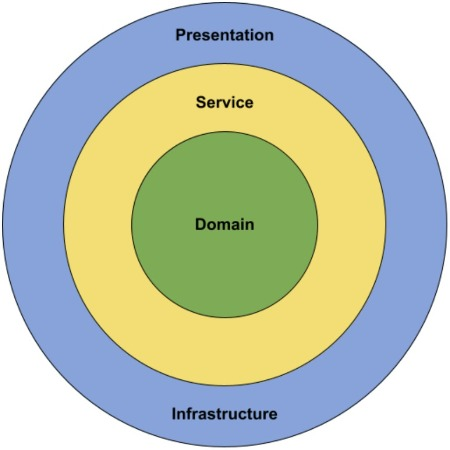
\includegraphics[width=.65\textwidth]{images/PrAR-Grundlagen-OnionArchitecture.jpeg}
    \caption{Bild Onion Architecture, nach \autocite{CodeMaze2024}}
    \label{fig:grundlagen:swdesign:onion}
\end{figure}

\newpage

Die Onion-Architecture gliedert sich in vier Hauptschichten:

\begin{itemize}
\item \textbf{Domain Layer:} Im Zentrum steht die Domäne, die Geschäftslogik und Geschäftsregeln beinhaltet und keinerlei Abhängigkeiten zu äußeren Schichten hat.
\item \textbf{Service Layer:} Diese Schicht enthält die Anwendungsspezifische Logik und nutzt die in der Domain Layer definierten Schnittstellen.
\item \textbf{Infrastructure Layer:} Hier befinden sich Implementierungen für Datenzugriff, Netzwerkkommunikation und andere externe Dienste.
\item \textbf{Presentation Layer:} Diese Schicht ist für die Benutzeroberfläche und die Präsentation der Daten verantwortlich.
\end{itemize}

Konzepte der Onion-Architecture fördern die Abhängigkeit von Abstraktionen (Interfaces) anstatt von konkreten Implementierungen. Diese Abhängigkeitsinversion erlaubt es, Implementierungen zur Laufzeit auszutauschen, was die Flexibilität und Erweiterbarkeit der Software erhöht.

Die Vorteile der Onion-Architecture sind:

\begin{itemize}
\item \textbf{Hohe Testbarkeit:} Da alle Schichten über definierte Schnittstellen kommunizieren, können einzelne Komponenten leicht isoliert und getestet werden.
\item \textbf{Klare Abhängigkeiten:} Abhängigkeiten fließen strikt in Richtung der zentralen Domänenschicht, wodurch höhere Schichten die Implementierungen der unteren Schichten verwenden können, aber nicht umgekehrt.
\item \textbf{Trennung von Geschäftslogik und Implementierungsdetails:} Die Geschäftslogik kann unabhängig von technischen Implementierungsdetails entwickelt werden. Notwendige Schnittstellen zu externen Systemen werden definiert, aber deren konkrete Implementierung wird in den äußeren Schichten gekapselt.
\end{itemize}

Diese Struktur ermöglicht es, komplexe Anwendungen modular zu entwickeln und erleichtert die Wartung und Weiterentwicklung der Software \autocite{CodeMaze2024}.

\subsection{Kollaboration mehrerer Dienste}

\subsubsection{Eventbasierte Architektur: Message Broker und Message Bus} \label{cha:grundlagen:swdesign:kollab:msgbus}

Eine eventbasierte Architektur ermöglicht es, Nachrichten schnell und flexibel zwischen mehreren Diensten auszutauschen. Ein verbreiteter Ansatz hierfür ist die Nutzung eines \textit{Message-Brokers}. Im Folgenden werden die vier grundlegenden Aspekte dieser Architektur beschrieben (vgl. \autocite{oreilly:mod-swarch}):
\begin{enumerate}
    \item \textbf{Initiierendes Event}: Ein \textit{Ereignis}, das den Event-Fluss anstößt und an einen Event-Kanal des Event-Brokers gesendet wird.
    \item \textbf{Event-Broker}: Ein \textit{Orchestrator}, der mehrere Kanäle verwaltet, auf denen Event-Prozessoren lauschen können.
    \item \textbf{Event-Prozessor}: Eine Einheit, die auf einem Kanal lauscht und ein eingehendes Event verarbeitet. Dabei kann ein neues (verarbeitetes) Event erzeugt und an einen anderen Kanal gesendet werden.
    \item \textbf{Das zu verarbeitende Event}: Ein Ereignis, das durch die beschriebenen Mechanismen verarbeitet oder erzeugt wird.
\end{enumerate}

\textbf{Vorteile}

\begin{enumerate}
    \item \textbf{Architektonische Erweiterbarkeit}: Events können vorläufig erzeugt und an den Message-Broker gesendet werden, ohne dass der Event-Prozessor bereits implementiert sein muss. Dies ermöglicht die spätere Implementierung des Prozessors.
    \item \textbf{Abkapselung}: Jedes Modul ist für seine eigene Funktionalität verantwortlich, während alles außerhalb Bestandteil anderer Module ist.
    \item \textbf{Skalierbarkeit}: Events können von mehreren (gleichen) Event-Prozessoren verarbeitet werden. Der Kanal fungiert als FIFO-Warteschlange und ermöglicht eine notwendige Synchronisation.
    \item \textbf{Asynchronität}: Die Kommunikation erfolgt asynchron, was die Entkopplung der Dienste und die Verbesserung der Systemleistung ermöglicht.
\end{enumerate}

\textbf{Nachteile}

\begin{enumerate}
    \item \textbf{(De-)Marshalling}: Nachrichten müssen in ein anderes Format (z.B. JSON, String, Byte-Array) konvertiert und wieder zurückkonvertiert werden. Dies kann die Performance beeinträchtigen.
    \item \textbf{Policies}: In einer traditionellen Message-Broking-Architektur kann theoretisch jeder auf einen Kanal \textit{subscriben}. Es gibt keine klaren Schichten zur Trennung der Zugriffsrechte.
    \item \textbf{Komplexität}: Das Management mehrerer Module und die Nachverfolgung von \textit{Event-Publishern} und \textit{Event-Subscriber} können schwierig sein.
\end{enumerate}

\subsubsection{RESTful APIs} \label{cha:grundlagen:collaboration:rest}

Für die Kommunikation und den Datenaustausch zwischen mehreren Diensten stehen verschiedene Kommunikations-Protokolle zur Verfügung. HTTP ist ein standardisiertes Kommunikationsprotokoll und ist in Bereichen der Web-Anwendungen weit verbreitet.

\ac{rest} definiert kein neues Kommunikationsprotokoll. Es ist ledigliche eine Sammlung von Architekturbeschränkungen und definiert Regeln, die der Entwickler befolgen muss, um eine Zustandslosigkeit in der Kommunikation zu erfüllen \autocite{RedHat2023}.


\section{Technologien}

Für die Implementierung wurden zahlreiche Technologien der Software-Entwicklung in Betracht gezogen. In diesem Abschnitt werden die für das Projekt relevanten Frameworks und Plattformen beschrieben.

\subsection{ASP.NET}

ASP.NET ist ein Open-Source-Web-Framework, das von Microsoft entwickelt wurde und die Erstellung moderner, skalierbarer und leistungsfähiger Webanwendungen ermöglicht. Zudem werden in ASP.NET moderne Webtechnologien und -standards unterstützt, wodurch sich die Entwicklung von interaktiven und responsiven Webanwendungen erleichtert. Dies schließt auch Apis und Echtzeit-Kommunikation ein, die für die Anwendung relevant sein könnten. Diese Merkmale ermöglichen es auch, die Anwendung modular zu ergänzen, indem externe Apis wie OpenStreetMaps oder andere Dienste einfach angebunden werden können. \autocite{MicrosoftLearn:AspNet}

\subsubsection{Entity Framework Core}

\ac{efcore} ist ein leichtgewichtiges, erweiterbares und Open-Source-\ac{orm} Framework für .NET, das entwickelt wurde, um den Datenzugriff und die Datenmanipulation in .NET-Anwendungen zu vereinfachen. \ac{efcore} bietet Datenbankunabhängigkeit, da es verschiedene Datenbanksysteme wie SQL Server, MySQL, PostgreSQL und SQLite unterstützt.

Ein weiterer Vorteil von \ac{efcore} ist Möglichkeit, das Datenbankschema aus konkreten Models über Source-Code zu generieren, ohne \textit{Create-Table} SQL-Statements schreiben zu müssen. \ac{efcore} bietet hierbei eine einfach zu verstehende \textit{Fluent-Api} an. Zudem ermöglicht \ac{efcore} die einfache Verwaltung von Datenbankmigrationen, was es erlaubt, Änderungen am Datenmodell nachzuverfolgen und auf die Datenbank anzuwenden. Dies erleichtert die Wartung und Weiterentwicklung erheblich.

Ein zusätzliches Merkmal von \ac{efcore} ist die Integration von \ac{linq}, die es ermöglicht, komplexe Abfragen auf eine intuitive und typsichere Weise zu schreiben. Dies verbessert die Lesbarkeit und Wartbarkeit des Codes erheblich. Schließlich bietet \ac{efcore} verschiedene Mechanismen zur Performanceoptimierung, wie zum Beispiel asynchrone Abfragen und Caching-Strategien. \autocite{MicrosoftLearn:EfCore}

\subsection{Unity und Mobile-Apps}

Unity ist eine Plattform zur Entwicklung und Darstellung interaktiver 3D-Inhalte, die in vielen Bereichen wie Spieleentwicklung, Filmproduktion, Architekturvisualisierung und \ac{vr} eingesetzt wird. Sie ist eine der am weitesten verbreiteten Spiel-Engines weltweit und bietet eine Vielzahl an Werkzeugen und Funktionen, für das implementieren immersiver und realistischer Umgebungen.

Unity basiert auf einer Engine, die eine umfassende Sammlung von Software-Bibliotheken bereitstellt. Diese Bibliotheken ermöglichen die Verarbeitung von Grafiken, Physik, Sound und Benutzereingaben. Der Kern der Engine ist für die Rendern von 2D- und 3D-Grafiken verantwortlich, die in Echtzeit berechnet und auf dem Bildschirm angezeigt werden. Unity unterstützt die Programmiersprachen C\# und UnityScript (eine Art JavaScript, welche allerdings nicht mehr weiterentwickelt wird), wobei C\#  die primäre Sprache für die Entwicklung in Unity ist. \autocite{UnityDocs2024}

\subsubsection{AR-Foundation}

Für das Erstellen von Augmented-Reality Anwendungen bietet Unity unter der \textit{AR Foundation} grundlegende Bausteine an. Über vorgefertigte Projekt-Templates lässt sich eine funktionierende und ausführbare Demo-Anwendung für Android-Geräte generieren. Das AR Foundation Framework ermöglicht das Einbinden von Features wie beispielsweise Oberflächen-Erkennung, Objekt-, Bild- und Gesicht-Verfolgung sowie Sitzungs- und Geräte-Management. \autocite{Unity2024}

\subsubsection{Nützliche Bibliotheken}

\textit{Newtonsoft.Json.NET} ist eine in der Praxis verwendete Bibliothek in C\# bzw. .NET Anwendungen für das Serialisieren und Deserialisieren von Objekten im JSON-Format. Für die Verwendung in Unity-Anwendungen existiert ein GitHub-Fork (\textit{Json.Net.Unity3D}) und ermöglicht das Einbinden über eine \lstinline{.unitypackage} Datei. \autocite{SaladLab2024}

\textit{AR+GPS Location} ist eine Utility aus dem Unity-Asset-Store und ermöglicht eine Übersetzung von GPS-Koordinaten im Unity-Raum. Hierdurch können Objekte über die Angabe eines realen GPS-Standorts im Unity-Raum plaziert werden. Wenn die Anwendung an der realen Stelle des angegebenen GPS-Standorts geöffnet wird, wird das in Unity angelegte Objekt am richtigen Ort angezeigt. \autocite{ArGpsLocation}

\subsection{Svelte und Web-Apps} \label{cha:grundlagen:swtech:svelte}

\textbf{Svelte} ist ein modernes JavaScript-Framework zur Erstellung von Benutzeroberflächen. Im Gegensatz zu herkömmlichen Frameworks wie React oder Vue, die den Großteil ihrer Arbeit im Browser erledigen, verlagert Svelte diese Arbeit in die Kompilierungsphase. Das bedeutet, dass der Code während des Build-Prozesses in effizientes, optimiertes JavaScript umgewandelt wird, das direkt im Browser ausgeführt wird. Dadurch wird die Laufzeitlast erheblich reduziert, was zu einer besseren Performance und kürzeren Ladezeiten führt. \autocite{Svelte2024}

Ein wesentlicher Vorteil von Svelte ist seine einfache Syntax, die es Entwicklern ermöglicht, reaktiven Code zu schreiben, ohne auf komplexe Zustandsverwaltungslösungen zurückgreifen zu müssen. Die Komponenten von Svelte bestehen aus HTML, CSS und JavaScript, was die Lernkurve für neue Benutzer verkürzt und die Entwicklungserfahrung vereinfacht. \autocite{Svelte2024}

\textbf{SvelteKit} ist ein Framework zur Erstellung von Svelte-Anwendungen. Es erweitert die Möglichkeiten von Svelte, indem es zusätzliche Werkzeuge und Funktionen bereitstellt, die speziell für die Entwicklung komplexer, leistungsstarker Webanwendungen benötigt werden. SvelteKit vereinfacht die Einrichtung und Strukturierung von Projekten und bietet Funktionen wie Routing, \ac{ssr}, statische Seitengenerierung und eine integrierte Entwicklungsumgebung. \autocite{Svelte2024}

\subsubsection{Vorteile}

Svelte integriert CSS-Styles direkt in die Komponenten mittels \textit{<style>-Tags}. Dadurch entfällt die Notwendigkeit einer zusätzlichen Konfiguration. Alternativ kann auf bestehende CSS-Bibliotheken wie TailwindCSS zurückgegriffen werden. Standardmäßig werden Styles scoped erstellt, um Konflikte zwischen Komponenten zu vermeiden. Dies sorgt für eine sichere und wartbare Codebasis der einzelnen Komponenten durch reduzierte Abhängigkeiten. Svelte verfügt über eingebaute Barrierefreiheitsprüfungen (\textit{Accessibility-Linting}), die auf offensichtliche und auch komplexere Probleme hinweisen. Dies hilft Entwicklern, von Anfang an barrierefreie Anwendungen zu erstellen. \autocite{SvelteExperienceBespoyasov}

Svelte-Pages verfügen standardmäßig über ein einfaches Prerendering, das durch Setzen eines Attributs gesteuert werden kann. SvelteKit bietet auch einfache Einstellungen, um verschiedene Startpfade für das Prerendering zu definieren, was die Flexibilität bei der Konfiguration erhöht. \autocite{SvelteExperienceBespoyasov}

Ein weiteres zentrales Feature von Svelte ist die Reaktivität. Durch die Definition sogenannter \textit{Reactive Statements} kann ein Ablauf beschrieben werden, der ausgeführt wird, wenn eine Abhängigkeit innerhalb dieses Blocks aktualisiert wird. Dies erleichtert das Management von Zustandsänderungen und ermöglicht reaktive und dynamische Benutzerschnittstellen. \autocite{SvelteExperienceBespoyasov}

Die deklarative Natur von Svelte reduziert die Menge des benötigten Codes erheblich. Dies führt zu einer übersichtlicheren Codebasis, welche die Entwicklung und Wartung von Anwendungen vereinfacht.\autocite{SvelteExperienceBespoyasov}

\subsubsection{Nachteile}

Im Vergleich zu bekannteren JavaScript-Frameworks wie React oder Angular ist die Community von Svelte aufgrund der Neuheit des Frameworks noch relativ klein. Dies kann die Fehlersuche erschweren, da einige Bugs möglicherweise nicht so gut dokumentiert oder gelöst sind und somit weniger Ressourcen in Foren wie Stack Overflow zur Verfügung stehen. \autocite{SvelteVsSvelteKit2023}

Ein weiterer Nachteil ist das Fehlen von Entwicklertools oder einer \ac{cli}. Bei Angular können beispielsweise Komponenten oder Services schnell und effizient mit dem Angular \ac{cli} erstellt werden. Diese Art von Tooling fehlt bei Svelte, was den Entwicklungsprozess etwas weniger komfortabel machen kann. \autocite{SvelteVsSvelteKit2023}

Darüber hinaus ist die Verfügbarkeit und Nutzbarkeit der vorhandenen Bibliotheken eingeschränkt. Zwar können diese Bibliotheken problemlos mit einem Paketmanager (z.B. npm von Node.js) installiert werden, jedoch ist es oft mit zusätzlichem Aufwand verbunden, diese in Svelte-Komponenten zu integrieren.\autocite{SvelteVsSvelteKit2023}

\subsubsection{Pages \& Routes}

Eine Svelte-Anwendung ist verzeichnisbasiert. Jedes Verzeichnis entspricht einer Route und kann ein oder mehrere Unterverzeichnisse haben, die die Route erweitern. Jede Route kann eine Seite haben, die immer \textit{+page.svelte} heißt. Svelte verwendet diese Seiten als Hauptanzeige, wenn zu der entsprechenden Route navigiert wird.

\subsubsection{UI Components}

Für die Darstellung, Wiederverwendbarkeit und Konsistenz zwischen verschiedenen Seiten werden Svelte-Komponenten verwendet. Diese bilden die Bausteine für die Darstellung unterschiedlicher Daten. Zusätzlich können UI-Komponentenbibliotheken wie z.B. \textit{flowbite-svelte} eingebunden werden, um standardisierte und ansprechende UI-Elemente wie Buttons, Inputs oder Tabellen zu implementieren. Die Verwendung einer vorgefertigten Bibliothek vereinfacht zudem die Entwicklung und trägt zu einer konsistenten und intuitiven Benutzererfahrung bei.

Jede Svelte-Komponente besteht aus einem Skriptteil und einem Design-/Styleteil. Eine Komponente kann auch andere Komponenten einbinden. In diesem Fall fungiert die übergeordnete Komponente als Elternteil (Parent), während die eingebetteten Komponenten als Kinder (Children) bezeichnet werden.

\subsubsection{Stores}

Um während des Erstellungs- und Bearbeitungsprozesses Daten zu speichern, wird ein Svelte Store verwendet. Dies ermöglicht es verschiedenen Komponenten, auf diese Daten zuzugreifen.

\subsubsection{Node \& Node Modules}

\textit{Node.js} ist eine JavaScript-Laufzeitumgebung, die serverseitige Anwendungen ermöglicht. Sie stellt über den Paketmanager \textit{npm} Werkzeuge zur Verwaltung und Bereitstellung von externen Paket-Abhängigkeiten sowie Entwickler-Tools bereit. Neben dem Betrieb eines Webservers ermöglicht \textit{Node.js} auch die serverseitige Verarbeitung von Api-Anfragen und die Anbindung an Datenbanken.

\subsection{Docker} \label{cha:grundlagen:swtech:docker}

Docker ist eine Technologie zum Deployment von Anwendungen (z.B. Dienste oder Datenbankverbindungen), die zu Testzwecken in der Entwicklungsphase eingesetzt werden können. Docker-Compose und Dockerfiles können ebenfalls zum Deployment von Anwendungen und Systemen verwendet werden.

\chapter{Problemanalyse} \label{cha:problemanalyse}

\section{Anforderungen und Problemabgrenzung} \label{cha:problemanalyse:abgrenzung}

Die Schnitzeljagden sollen in erster Linie den Studienanfängern dienen, um ihnen auf interaktive Weise den Campus nahe zu bringen und sie mit den wichtigsten Orten und Einrichtungen vertraut zu machen.

Im Rahmen des Projekts wurden folgende Ziele in einer Vier-Felder-Matrix aufgeteilt.

\begin{figure}[H]
    \centering
    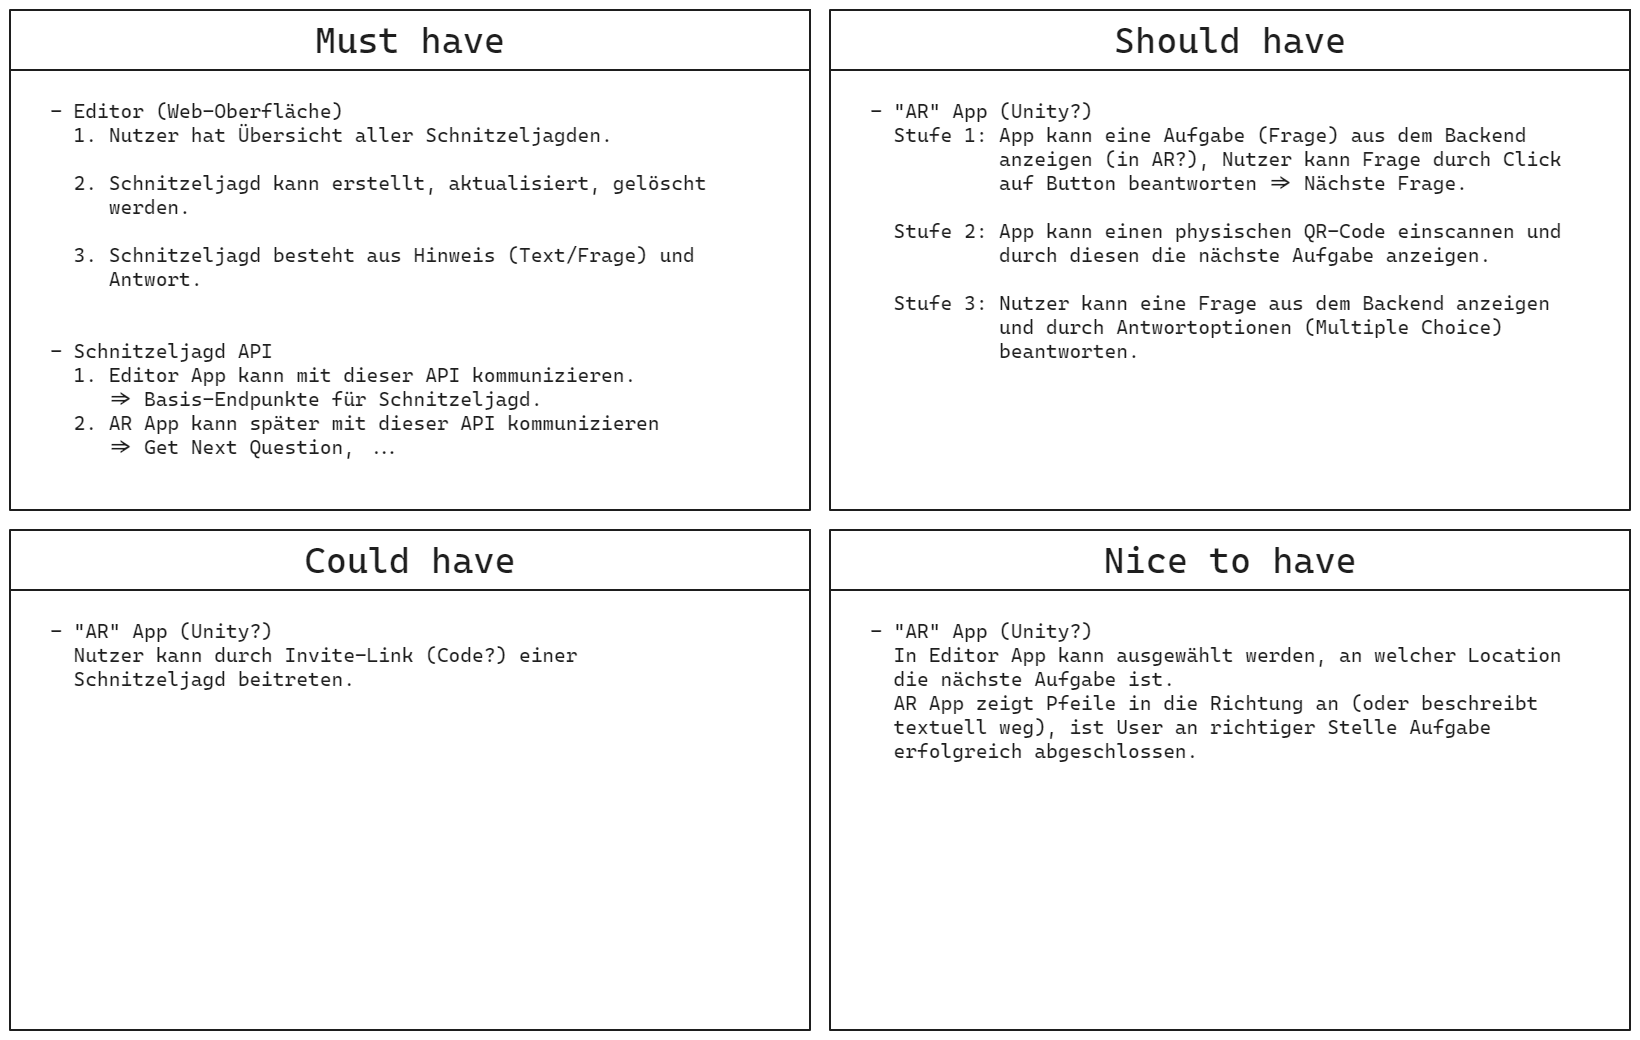
\includegraphics[width=\textwidth]{images/PrAr_ProblemAnalysis_Vierfelder.png}
    \caption{Darstellung der Projekt-Ziele aufgeteilt in Vier Felder}
    \label{fig:problemanalyse:vierfeldermatrixamarsch}
\end{figure}

Für die erfolgreiche Projektumsetzung sind folgende Eigenschaften zu berücksichtigen.

\subsubsection{Flexibilität}

Ein wichtiger Aspekt des Projektes ist, dass eine Schnitzeljagd so flexibel wie möglich umgesetzt werden soll. Aufgabenstellung und Lösung sollen voneinander entkoppelt und ohne großen Implementierungsaufwand dynamisch erweiterbar sein.

\subsubsection{Skalierbarkeit}

Das System muss in der Lage sein, mehrere Schnitzeljagden gleichzeitig ohne Probleme durchzuführen. Es sollte möglich sein, die Ressourcen des Systems dynamisch an die Anzahl der gerade aktiven Benutzer anzupassen, ohne dass es zu Leistungseinbußen oder ähnlichen Beeinträchtigungen kommt.

\subsubsection{Benutzerfreundlichkeit}

Der Anmelde- und der Durchführungsprozess sollten unabhängig voneinander klar strukturiert sein, um den Benutzern eine reibungslose und intuitive Erfahrung zu bieten. Während der Schnitzeljagd sollten keine Schwierigkeiten auftreten. Die Schnitzeljagd sollte den Benutzern ein einzigartiges Erlebnis bieten, ohne sie durch unnötige oder ablenkende Elemente zu stören. Idealerweise fungiert die Anwendung als Schnittstelle zur Durchführung der Schnitzeljagd, wobei die Lösung der Aufgaben direkte Interaktionen im realen Leben erfordert.

Die digitale Plattform ermöglicht eine einfache Anmeldung und Durchführung der Schnitzeljagd, wodurch der organisatorische Aufwand minimiert und die Zugänglichkeit maximiert wird.

\subsubsection{Sicherheit}

Das Thema Sicherheit ist im Zusammenhang mit sensiblen Benutzerdaten wie Passwörtern sehr wichtig. Durch die im Kapitel \ref{cha:swentwurf} beschriebenen Architekturüberlegungen wäre es möglich, Benutzerdaten durch kryptographisch sichere Hashfunktionen zu speichern. Um den Projektumfang auf das Wesentliche zu reduzieren, wurde dies im Projekt nicht berücksichtigt.

\section{Architektonische Überlegungen}

Bei der Wahl einer angemessenen Architektur für das System sind viele Aspekte zu berücksichtigen, unter anderem die in Kapitel \ref{cha:problemanalyse:abgrenzung} genannten Eigenschaften.

In Kapitel \ref{cha:swentwurf} wird daher der service-orientierte Ansatz für den Entwurf der Software allumfassend beschrieben.


\chapter{Software-Entwurf} \label{cha:swentwurf}

\section{Blockansicht}

Im folgenden ist die Struktur (\textit{High-Level-Ansicht}) des Software-Systems in Form eines Blackbox-Diagrams dargestellt.

\begin{figure}[H]
    \centering
    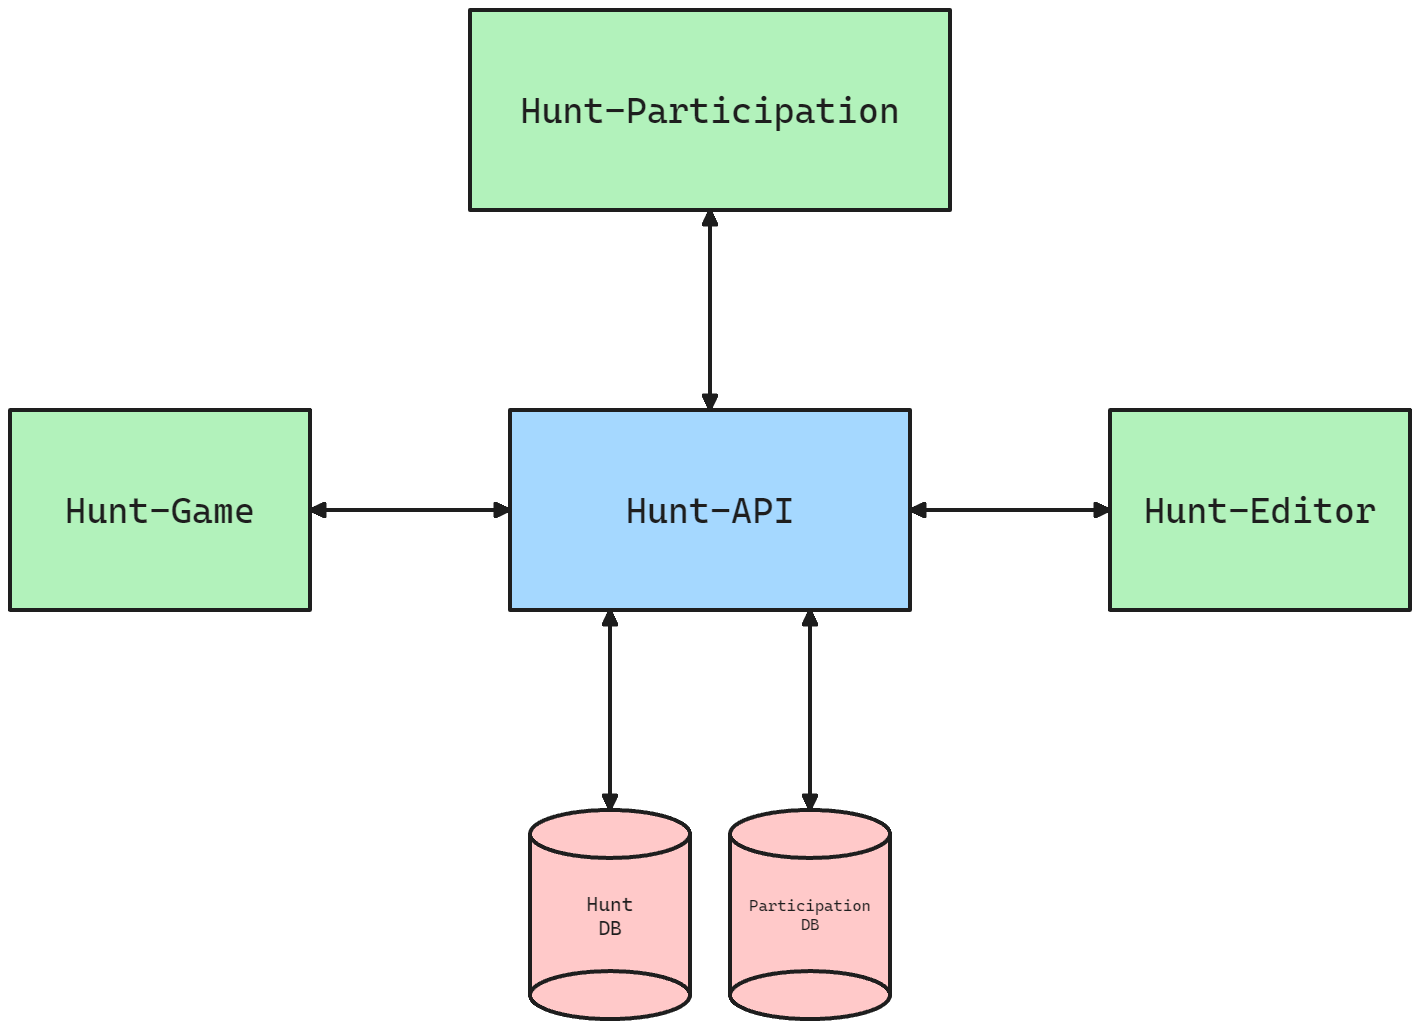
\includegraphics[width=\textwidth]{images/PrAr-Software-Entwurf-Blockansicht.png}
    \caption{Bild Systemkontext als Blackbox-Diagram}
    \label{fig:swentwurf:blackbox}
\end{figure}

Das in Abbildung \ref{fig:swentwurf:blackbox} dargestellte Blackbox-Diagramm beschreibt den Zusammenhang der unterschiedlichen Subsysteme zueinander. Die verschiedenen Aufgaben, die das System zu leisten hat, wurden als einzelne Anwendungen vorhergesehen. Diese sind in Abbildung \ref{fig:swentwurf:blackbox} grün markiert. Dies ermöglicht eine klare Trennung der verschiedenen Domänen (Erstellung, Anmeldung, Durchführung). Das Backend steht als zentrale Schnittstelle für die Bereitstellung systemspezifischer Funktionalitäten zur Verfügung. Dieses sind in Abbildung \ref{fig:swentwurf:blackbox} blau markiert. Für die Datenpersistierung besitzt das Backend zwei Datenbank-Verbindungen. Dieses sind in Abbildung \ref{fig:swentwurf:blackbox} rot markiert.

\section{Hunt-Api Backend} \label{cha:swentwurf:backend}

\subsection{Übersicht}

Anhand einer zentral zur Verfügung stehenden Schnittstelle \textit{Hunt-Api} können die verschiedenen Anwendungen zur Gesamt-Funktionalität des Systems beitragen. Die Schnittstelle bietet verschiedene Endpunkte für die Verwaltung von Schnitzeljagden, Teilnahmen und die bewältigten Aufgaben der Teilnehmer. Eine Darstellung der Hunt-Api Architektur ist in Abbildung \ref{fig:swentwurf:huntapi:subsystem} näher beschrieben.

\begin{figure}[H]
    \centering
    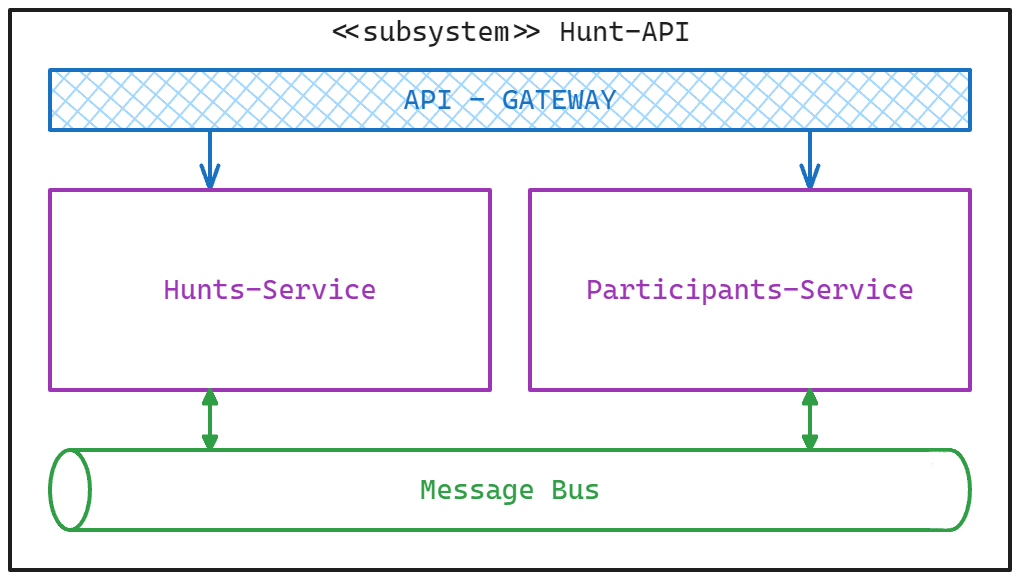
\includegraphics[width=\textwidth]{images/PrAr-Software-Entwurf-Hunt-Api-Subsystem.png}
    \caption{Bild Hunt-Api Subsystem}
    \label{fig:swentwurf:huntapi:subsystem}
\end{figure}

Als Architekturmuster wurde ein domänenorientierter Ansatz gewählt, der in Kapitel \ref{cha:grundlagen:swdesign:ddd} näher erläutert wird. Jede Domäne repräsentiert dabei einen spezifischen Teilaspekt des Gesamtsystems. Die ausgewählten Domänen, \textit{Hunts} und \textit{Participants}, sind in Abbildung \ref{fig:swentwurf:huntapi:subsystem} lila hervorgehoben und repräsentieren den jeweiligen Dienst als Microservice (vgl. Kapitel \ref{cha:grundlagen:swdesign:microservices}).

Für die Kommunikation unterschiedlicher Dienste ist ein Message-Bus vorhergesehen (vgl. Kapitel \ref{cha:grundlagen:swdesign:kollab:msgbus}), worüber eventgesteuert Nachrichten ausgestauscht werden. Dieser ist in Abbildung \ref{fig:swentwurf:huntapi:subsystem} grün hervorgehoben. Wieso ein Message-Bus nötig ist, wird im Anhang \ref{appendix:adr:messagebus} näher beschrieben.

Um eine einheitliche Schnittstelle bereitzustellen, die anwendungsübergreifend genutzt werden kann, wurde ein Api-Gateway vorhergesehen. Hierrüber werden Anfragen an an den entsprechenden Dienst weitergeleitet. Das Api-Gateway ist in Abbildung \ref{fig:swentwurf:huntapi:subsystem} blau gekennzeichnet. Im Anhang \ref{appendix:adr:proxy} wird näher beschrieben, weshalb ein Api-Gateway gewählt wurde.

\subsection{Hunts-Service} \label{cha:swentwurf:huntsservice}

\subsubsection{Übersicht}

Für die Verwaltung der erstellten Schnitzeljagden eines Organisators, ist der Hunts-Service vorhergesehen. Abbildung \ref{fig:swentwurf:huntapi:huntservice} zeigt die Struktur des Dienstes.

\begin{figure}[H]
    \centering
    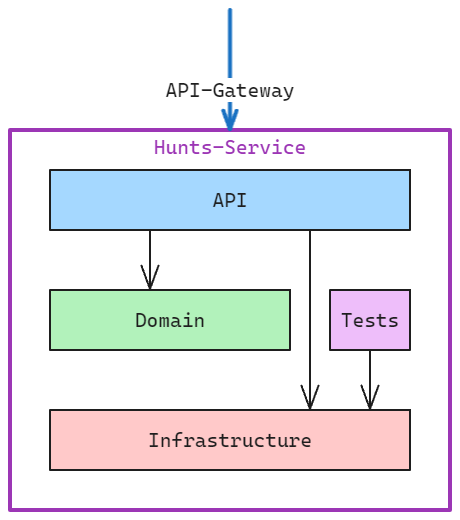
\includegraphics[width=0.6\textwidth]{images/PrAr-Software-Entwurf-Hunt-Api-Hunt-Service.png}
    \caption{Bild Hunts Microservice}
    \label{fig:swentwurf:huntapi:huntservice}
\end{figure}

Innerhalb des Hunts-Service wurde ein schichtenorientierter Ansatz gewählt, welcher Ähnlichkeiten mit der in Kapitel \ref{cha:grundlagen:swdesign:onion} beschriebenen \textit{Onion-Architecture} teilt. Jede Schicht entspricht einer horizontalen Teilung der unterschiedlichen Anwendungs-Aspekte. Für die Persistierung der Schnitzeljagden (Hunts) wurde das Repository-Pattern vorhergesehen.

Die grundlegende Funktionalität der Domäne (\textit{Hunts}, \textit{Assignments}, etc.) wird in der \textit{Domain-Schicht} zur Verfügung gestellt, welche in Abbildung \ref{fig:swentwurf:huntapi:huntservice} grün gekennzeichnet wird. Hier sind Modelle und Entities, sowie Datentypen, Enumerations und Repository-Interfaces definiert, die im System durchweg Verwendung finden. Die Domain-Schicht ist abgekapselt von Anwendungs- und Infrastrukturlogik und besitzt daher keine Abhängigkeiten zu externen Modulen.

Eine Implementierung der Repository-Interfaces wird in der \textit{Infrastruktur-Schicht} (Infrastructure) zur Verfügung gestellt, die in Abbildung \ref{fig:swentwurf:huntapi:huntservice} rot hervorgehoben wird. Diese kann zudem unabhängig von der Domänen-Logik isoliert getestet werden, wie in in Abbildung \ref{fig:swentwurf:huntapi:huntservice} lila dargestellt wird.

Die \textit{Anwendungs-Schicht} ist in Abbildung \ref{fig:swentwurf:huntapi:huntservice} blau hervorgehoben und bündelt die Funktionalität der Domain-Schicht und Infrastruktur-Schicht gemeinsam. Über eine einheitliche Schnittstelle (\textit{api/Hunt}) können Schnitzeljagden erstellt, bearbeitet, gelöscht und aufgelistet werden.

\subsubsection{Schnittstellendefinition}

\begin{figure}[H]
    \centering
    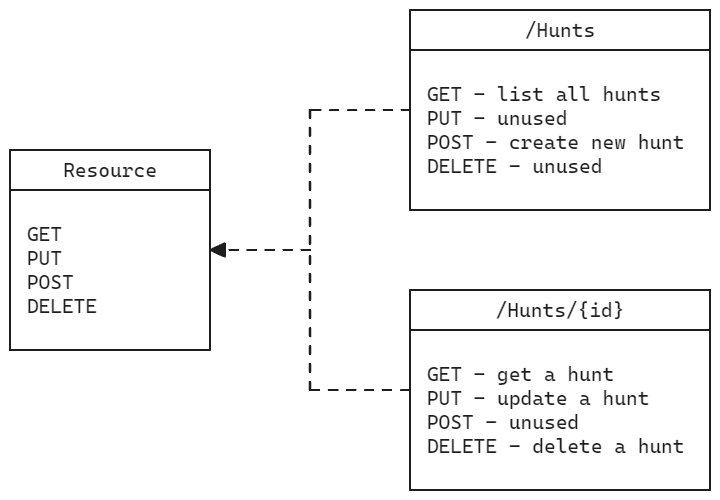
\includegraphics[width=0.6\textwidth]{images/PrAr-Software-Entwurf-Hunt-Api-Hunt-Service-Endpoints.png}
    \caption{Skizze der Hunts Ressourcenansicht}
    \label{fig:swentwurf:huntapi:huntservice:endpoints}
\end{figure}

In Abbildung \ref{fig:swentwurf:huntapi:huntservice:endpoints} sind die unterschiedlichen Operationen auf Schnitzeljagden (\textit{Hunts}) anhand des ressourcen-orientierten Ansatz aus Kapitel \ref{cha:grundlagen:collaboration:rest} dargestellt. Diese entspricht der tatsächlichen Schnittstelle, die für den Hunts-Service vorhergesehen wurde.

\subsubsection{Datenbank-Modell}

\begin{figure}[H]
    \centering
    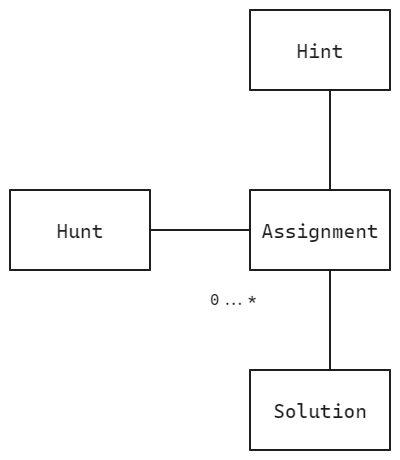
\includegraphics[width=0.6\textwidth]{images/PrAr-Software-Entwurf-Hunt-Api-Hunt-Service-Er.png}
    \caption{Skizze ER-Modell der Hunts}
    \label{fig:swentwurf:huntapi:huntservice:er}
\end{figure}

Abbildung \ref{fig:swentwurf:huntapi:huntservice:er} beschreibt das gewählte Entity-Relationship Diagram für das Datenbank-Modell des Hunts-Service.

\begin{itemize}
    \item \textbf{Hunt}: Die Schnitzeljagd. Enthält einen Titel, eine Beschreibung und eine Liste von 0 bis n Aufgaben (\textit{Assignments}).
    \item \textbf{Assignment}: Eine konkrete Aufgabe einer Schnitzeljagd. Besteht aus einem Hinweis (\textit{Hint}) und eine Lösung (\textit{Solution}).
    \item \textbf{Hint}: Ein Hinweis. Besteht aus einem Hinweis-Typ (als Enumeration) und den Hinweis-Daten als String.
    \item \textbf{Solution}: Eine Lösung zu einem gegebenen Hinweis. Besteht aus einem Lösungs-Typ (als Enumeration) und den Lösungs-Daten als String.
\end{itemize}

Wieso auf die Verwendung eines abtrakten Datenmodells verzichtet wurde, wird im Anhang \ref{appendix:adr:er} näher beschrieben.

\subsection{Participants-Service} \label{cha:swentwurf:participantsservice}

\subsubsection{Übersicht}

Damit ein Teilnehmer an einer Schnitzeljagd teilnehmen und diese auch durchführen kann, soll ihm die Anmelde- und Spielfunktionalität zur Verfügung gestellt werden. Dies wird über den Participants-Service ermöglicht. Abbildung \ref{fig:swentwurf:huntapi:participantservice} zeigt die Struktur des Dienstes.

\begin{figure}[H]
    \centering
    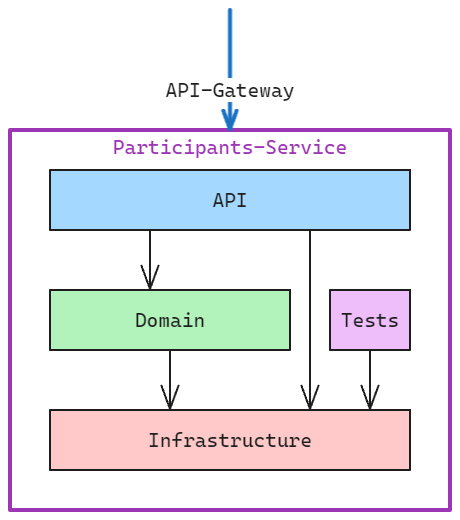
\includegraphics[width=0.6\textwidth]{images/PrAr-Software-Entwurf-Hunt-Api-Participant-Service.png}
    \caption{Bild Participants Microservice}
    \label{fig:swentwurf:huntapi:participantservice}
\end{figure}

Der Participants-Service besitzt eine ähnliche Struktur wie der Hunts-Service aus Kapitel \ref{cha:swentwurf:huntsservice} und erfüllt die Aufgabe der Teilnahmen-Verwaltung.

\subsubsection{Schnittstellendefinition}

\begin{figure}[H]
    \centering
    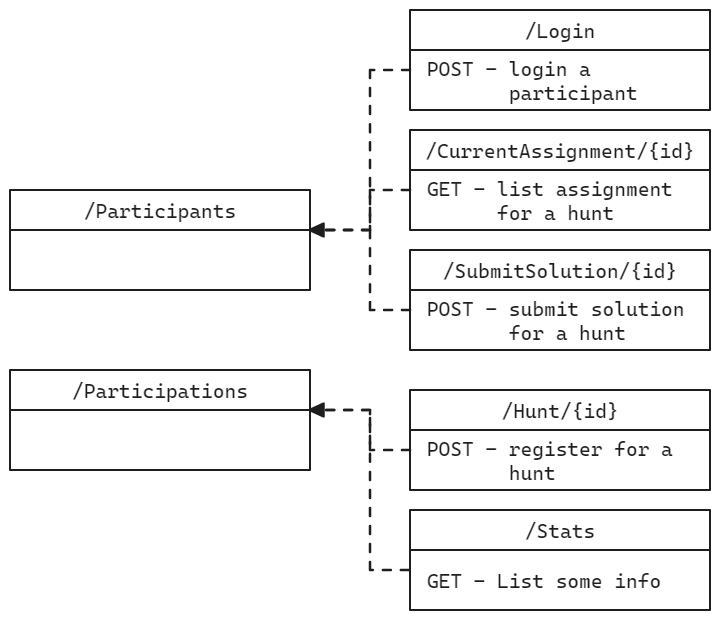
\includegraphics[width=0.6\textwidth]{images/PrAr-Software-Entwurf-Hunt-Api-Participant-Service-Endpoints.png}
    \caption{Skizze der Participants Schnittstelle}
    \label{fig:swentwurf:huntapi:participantservice:endpoints}
\end{figure}

Abbildung \ref{fig:swentwurf:huntapi:participantservice:endpoints} definiert die vorhergesehene Schnittstelle für den Participants-Service.

Unter dem Endpunkt \textit{Teilnehmer} wird dem Teilnehmer die Funktionalität zum \textit{Login} angeboten. Hierüber erhält er zusätzlich Informationen über die aktuell angemeldeten Schnitzeljagden. Möchte er eine entsprechende Schnitzeljagd starten oder fortsetzen, kann er dazu über \textit{Current-Assignment} den aktuellen Hinweis anfordern. Wenn der Teilnehmer dem Hinweis gefolgt ist und die Lösung gefunden hat, kann er diese dem System mit \textit{Submit-Solution} mitteilen. Das System stellt dann fest, ob die Lösung korrekt ist.

Der genaue Ablauf und das Zusammenspiel der einzelnen Endpunkte wird in Kapitel \ref{cha:swentwurf:spielablauf} erläutert.

Damit sich Teilnehmer für eine Schnitzeljagd anmelden können, ist unter dem Endpunkt \textit{Teilnahmen} mit \textit{Schnitzeljagd} und entsprechender \textit{Schnitzeljagd-ID} eine Registrierungsmöglichkeit vorgesehen. Zusätzlich können allgemeine Informationen wie z.B. die Anzahl der Teilnehmer oder die Anzahl aller Teilnahmen an Schnitzeljagden über den Endpunkt \textit{Stats} aufgelistet werden.

\subsubsection{Datenbank-Modell}

\begin{figure}[H]
    \centering
    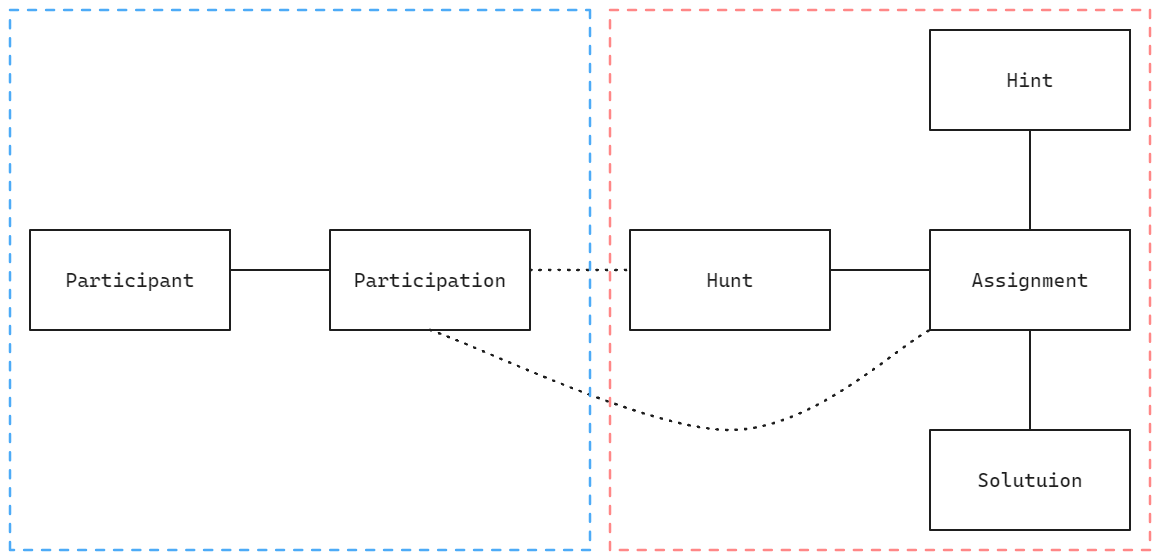
\includegraphics[width=0.6\textwidth]{images/PrAr_Software-Entwurf-Hunt-Api-Participant-Service-Er.png}
    \caption{Skizze ER-Modell zwischen Hunts und Participants}
    \label{fig:swentwurf:huntapi:participantservice:er}
\end{figure}

Abbildung \ref{fig:swentwurf:huntapi:participantservice:er} beschreibt das gewählte Entity-Relationship-Diagramm für das Datenbankmodell des Participants-Service. Die Teilnahmen (Participants und Participations) sollen relational gespeichert werden, während die Schnitzeljagden in einem nicht-relationalen Modell (z.B. Redis-Cache) gespeichert werden sollen, da diese bereits korrekt im Hunts-Service gespeichert werden (siehe Kapitel \ref{cha:swentwurf:huntsservice}).

\section{Hunt-Editor Web-App}

\subsection{Übersicht}

Mit dem Hunt-Editor kann der Organisator die Schnitzeljagden verwalten. Dazu startet er die Anwendung und gelangt auf das Dashboard. Hier erhält er einen Überblick über die erstellten Schnitzeljagden. Ihm wird die Funktion zum Erstellen (\textit{Create}) angeboten. Er kann Titel und Beschreibung sowie die jeweiligen Aufgaben mit Hinweis und Lösung anlegen und speichern. Die Reihenfolge der Aufgaben kann verändert werden.
\subsection{Wireframing}

Für die Entwicklung des Editors zur Erstellung und Verwaltung von Schnitzeljagden wurde zunächst der Wireframing-Ansatz verwendet. Wireframing ist eine wichtige Phase im Designprozess, die es ermöglicht, die Struktur und Funktionalität einer Anwendung visuell darzustellen, bevor mit dem detaillierten Design und der Entwicklung begonnen wird. In dieser frühen Planungsphase wird ein einfaches, oft schematisches Layout der Benutzeroberfläche erstellt, das die Anordnung der verschiedenen Elemente wie Schaltflächen, Menüs und interaktive Komponenten zeigt.

Im Folgenden werden die verschiedenen Wireframes vorgestellt und erläutert, warum sie eine solide Grundlage für die weitere Entwicklung des Editors bildeten, welche Stärken sie in Bezug auf Benutzerfreundlichkeit und Funktionalität aufwiesen und welche Schwächen oder Herausforderungen bei der Umsetzung erkannt wurden, die in späteren Phasen berücksichtigt werden mussten.

\begin{figure}[H]
  \centering
  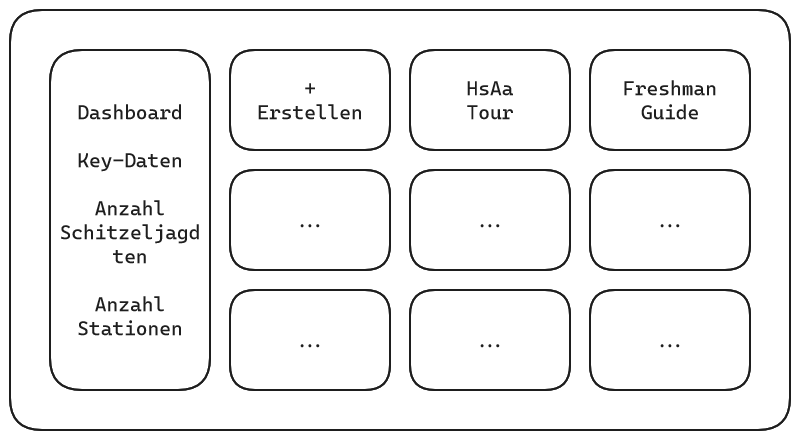
\includegraphics[width=1\textwidth]{images/wireframing/PrAr_Scavhunt_Wireframing-2.1.png}
  \caption{Skizze Dashboard des Hunt-Editors}
  \label{fig:wireframing-frontend-hunt-editor-3}
\end{figure}

Dies ist ein Wireframe, das relativ am Anfang der Entwicklungsphase erstellt wurde. Hier wurde ein Grid-Layout verwendet, um die Schnitzeljagd darzustellen. An der Seite befindet sich eine Sidebar, in der verschiedene Schlüsseldaten abgelesen werden können. Da es aber aufgrund der Architekturänderungen keine Stationen mehr gibt, fällt diese Information weg. Das Grid-Layout soll jedoch beibehalten werden.

\begin{figure}[H]
  \centering
  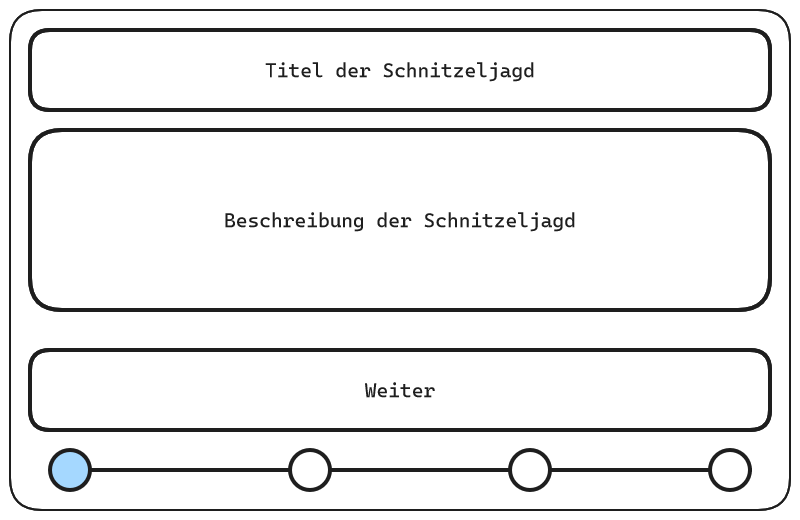
\includegraphics[width=1\textwidth]{images/wireframing/PrAr_Scavhunt_Wireframing-2.2.png}
  \caption{Skizze für Eingabe von Basisdaten im Hunt-Editor}
  \label{fig:wireframing-frontend-hunt-editor-4}
\end{figure}

Hier wird nun der Prozess der Erstellung einer Schnitzeljagd beschrieben, wobei uns die Verwendung eines Fortschrittsbalkens gefallen hat, der den aktuellen Stand der Erstellung anzeigt. Auch die Eingabe von Titel und Beschreibung sollte später so übernommen werden. 

\begin{figure}[H]
  \centering
  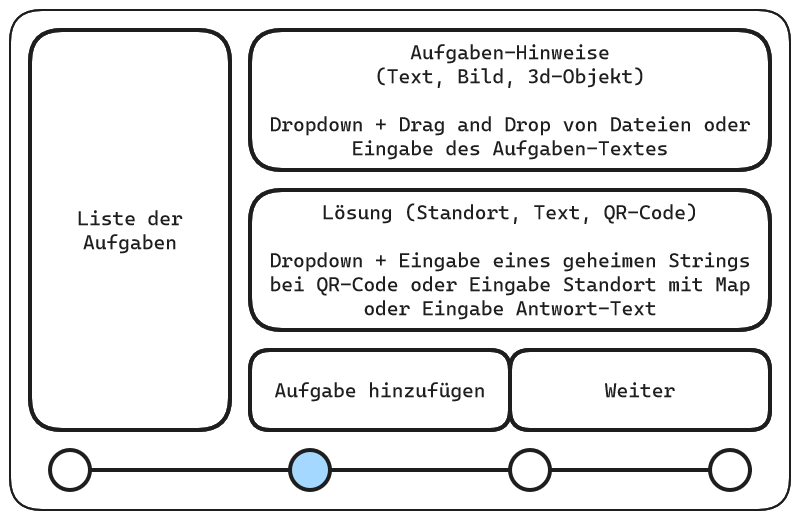
\includegraphics[width=1\textwidth]{images/wireframing/PrAr_Scavhunt_Wireframing-2.3.png}
  \caption{Skizze für Anlegen von Aufgaben im Hunt-Editor}
  \label{fig:wireframing-frontend-hunt-editor-5}
\end{figure}

Nun kommt der schwierigste Teil, die Erstellung und Bearbeitung der Aufgaben in einer Schnitzeljagd. Hier war zunächst der Ansatz, auf der linken Seite eine Tabelle mit den Aufgaben zu führen. Durch Anklicken der entsprechenden Zeile wird dann auf der rechten Seite die Aufgabe und die Lösung angezeigt. Hier gibt es auch noch den Aufgabentyp "3D-Objekt", der am Ende nicht übernommen wurde. 

\begin{figure}[H]
  \centering
  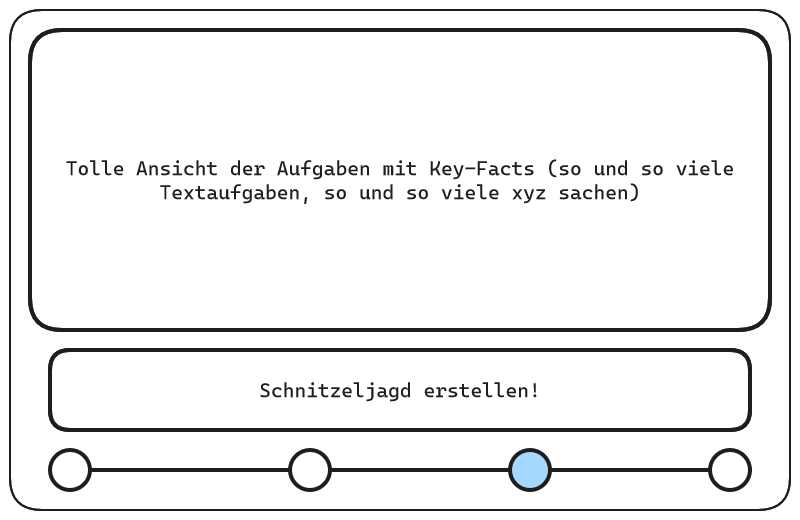
\includegraphics[width=1\textwidth]{images/wireframing/PrAr_Scavhunt_Wireframing-2.4.png}
  \caption{Skizze zur Übersicht einer Schnitzeljagd im Hunt-Editor}
  \label{fig:wireframing-frontend-hunt-editor-6}
\end{figure}

Dieses Wireframe zeigt am Ende noch einmal alle wichtigen Informationen der Schnitzeljagd im Überblick. Dieses Konzept hat uns gut gefallen. 

\begin{figure}[H]
  \centering
  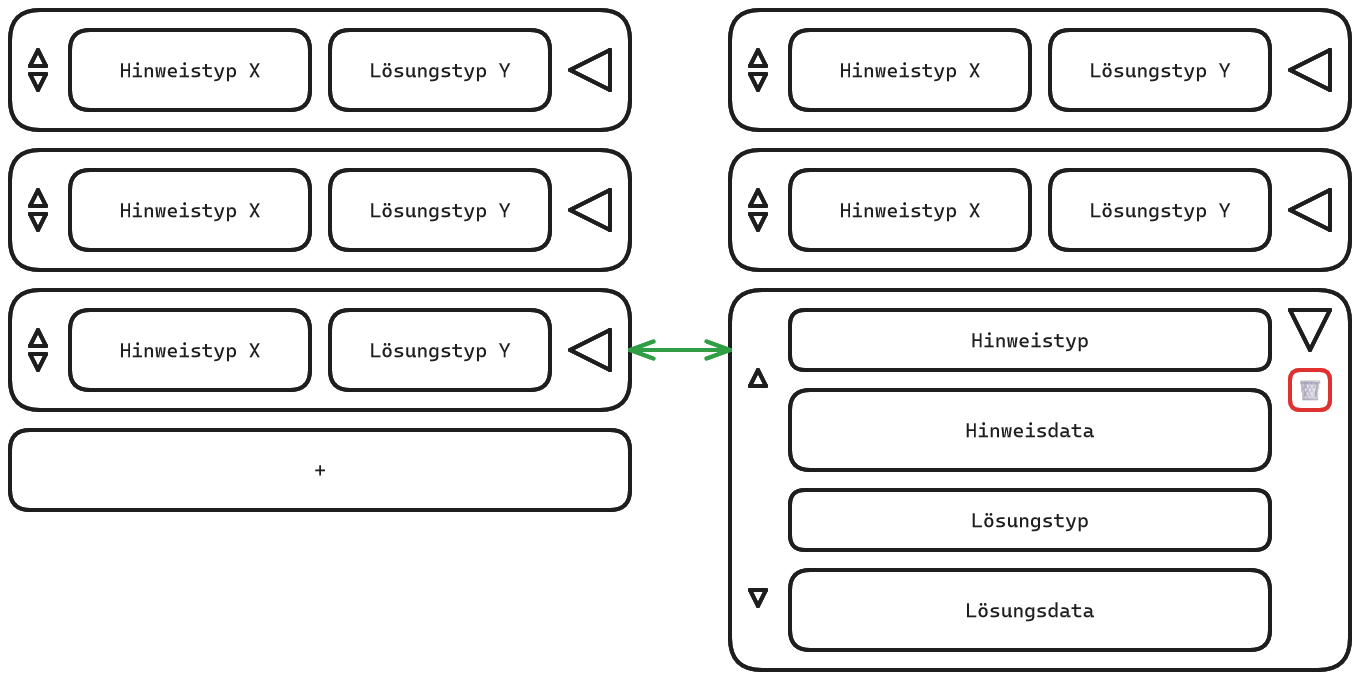
\includegraphics[width=1\textwidth]{images/wireframing/PrAr_Scavhunt_Wireframing-3.png}
  \caption{Skizze zur Auflistung von Aufgaben im Hunt-Editor}
  \label{fig:wireframing-frontend-hunt-editor-7}
\end{figure}

Da die seitliche Liste in Abbildung \ref{fig:wireframing-frontend-hunt-editor-5} für die Darstellung der Aufgaben auf mobilen Endgeräten ungeeignet ist, haben wir uns für den Ansatz in Abbildung \ref{fig:wireframing-frontend-hunt-editor-7} entschieden. Hier werden die Aufgaben nacheinander angezeigt und ihre Reihenfolge kann über die Pfeiltasten verändert werden. Um die Aufgaben zu bearbeiten, können diese über den Button auf der rechten Seite aufgeklappt und wieder zugeklappt werden. Im aufgeklappten Zustand befindet sich jeweils ein Dropdown für Aufgabe und Lösung sowie Eingabefelder / FileUpload oder eine Map-Integration für den Standort als Lösung. 

\section{Participation Web-App}

\subsection{Übersicht}

Über die Participation Web App kann sich ein Teilnehmer für eine Schnitzeljagd anmelden. Dazu startet er die Anwendung und gelangt auf eine Willkommensseite. Hier kann er sehen, wie viele Teilnehmer und wie viele Teilnahmen es insgesamt gibt. Um an einer Schnitzeljagd teilzunehmen, kann der Teilnehmer eine E-Mail an den Organisator schreiben. Wenn er daraufhin einen Einladungslink für eine Schnitzeljagd erhält, muss er dort nur noch einen Benutzernamen und ein Passwort auswählen. Mit diesem Benutzernamen und Passwort loggt er sich in das im Kapitel \ref{subsec:swentwurf:hunt-game} beschriebene Hunt-Game ein.

\subsection{Wireframing}

\begin{figure}[H]
  \centering
  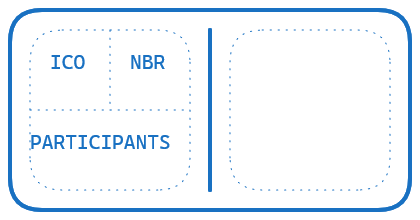
\includegraphics[width=1\textwidth]{images/PrAr_Scavhunt_Wireframing_Participant_1.png}
  \caption{Skizze zur Anzeige von Statistiken in der Participation Web-App}
  \label{fig:wireframing-frontend-participant-1}
\end{figure}

Um auf der Startseite der Participation Web-App interessante Statistiken anzeigen zu können, musste ein Konzept gefunden werden, wie diese ansprechend dargestellt werden können. Auf der linken Seite sollte die Anzahl aller Teilnehmer und auf der rechten Seite die Anzahl aller Beteiligungen dargestellt werden. Diese Informationen werden durch eine vertikale Trennlinie getrennt, um die verschiedenen Statistiken klar voneinander abzugrenzen.

\begin{figure}[H]
  \centering
  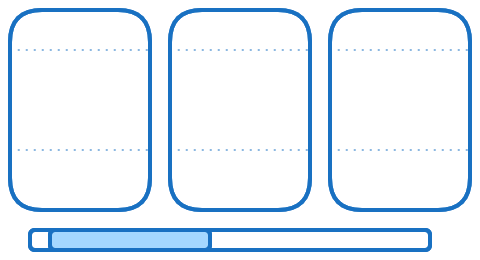
\includegraphics[width=1\textwidth]{images/PrAr_Scavhunt_Wireframing_Participant_2.png}
  \caption{Skizze zur Benachrichtigung eines Organisators in der Participation Web-App}
  \label{fig:wireframing-frontend-participant-2}
\end{figure}

Der Teilnehmer soll auch die Möglichkeit haben, einen Organisator um einen Einladungslink zu bitten. Dazu wurde das Wireframe erstellt, in dem die Organisatoren als Karten dargestellt werden. Hier kann auf mobilen Geräten durch horizontales Wischen zwischen den Organisatoren gewählt werden. 
\section{Hunt-Game Web-App} \label{subsec:swentwurf:hunt-game}

\subsection{Übersicht}
Beim Start der Anwendung sieht der Teilnehmer eine Sammlung von Bildern der Hochschule Aalen, darunter eine kleine Zeitleiste, die den Entwicklungsprozess der Projektarbeit beschreibt. Um an einer Schnitzeljagd teilnehmen zu können, muss sich der Teilnehmer mit dem gewählten Benutzernamen und Passwort der Participation Web-App anmelden. Anschließend wird ihm eine Übersicht aller Schnitzeljagden angezeigt, für die er sich registriert hat. Hierbei wird zwischen \textit{Ongoing, Complete} und \textit{Expired} unterschieden, was durch den aktuellen Teilnahme-Status bestimmt wird. Wählt er eine gültige Schnitzeljagd aus, startet der Spielablauf. 

\subsection{Spielablauf} \label{cha:swentwurf:spielablauf}

Abbildung \ref{fig:hunt_game_spielablauf} stellt den Spielablauf als UML-Programmablaufplan dar. 

\begin{figure}[H]
  \centering
  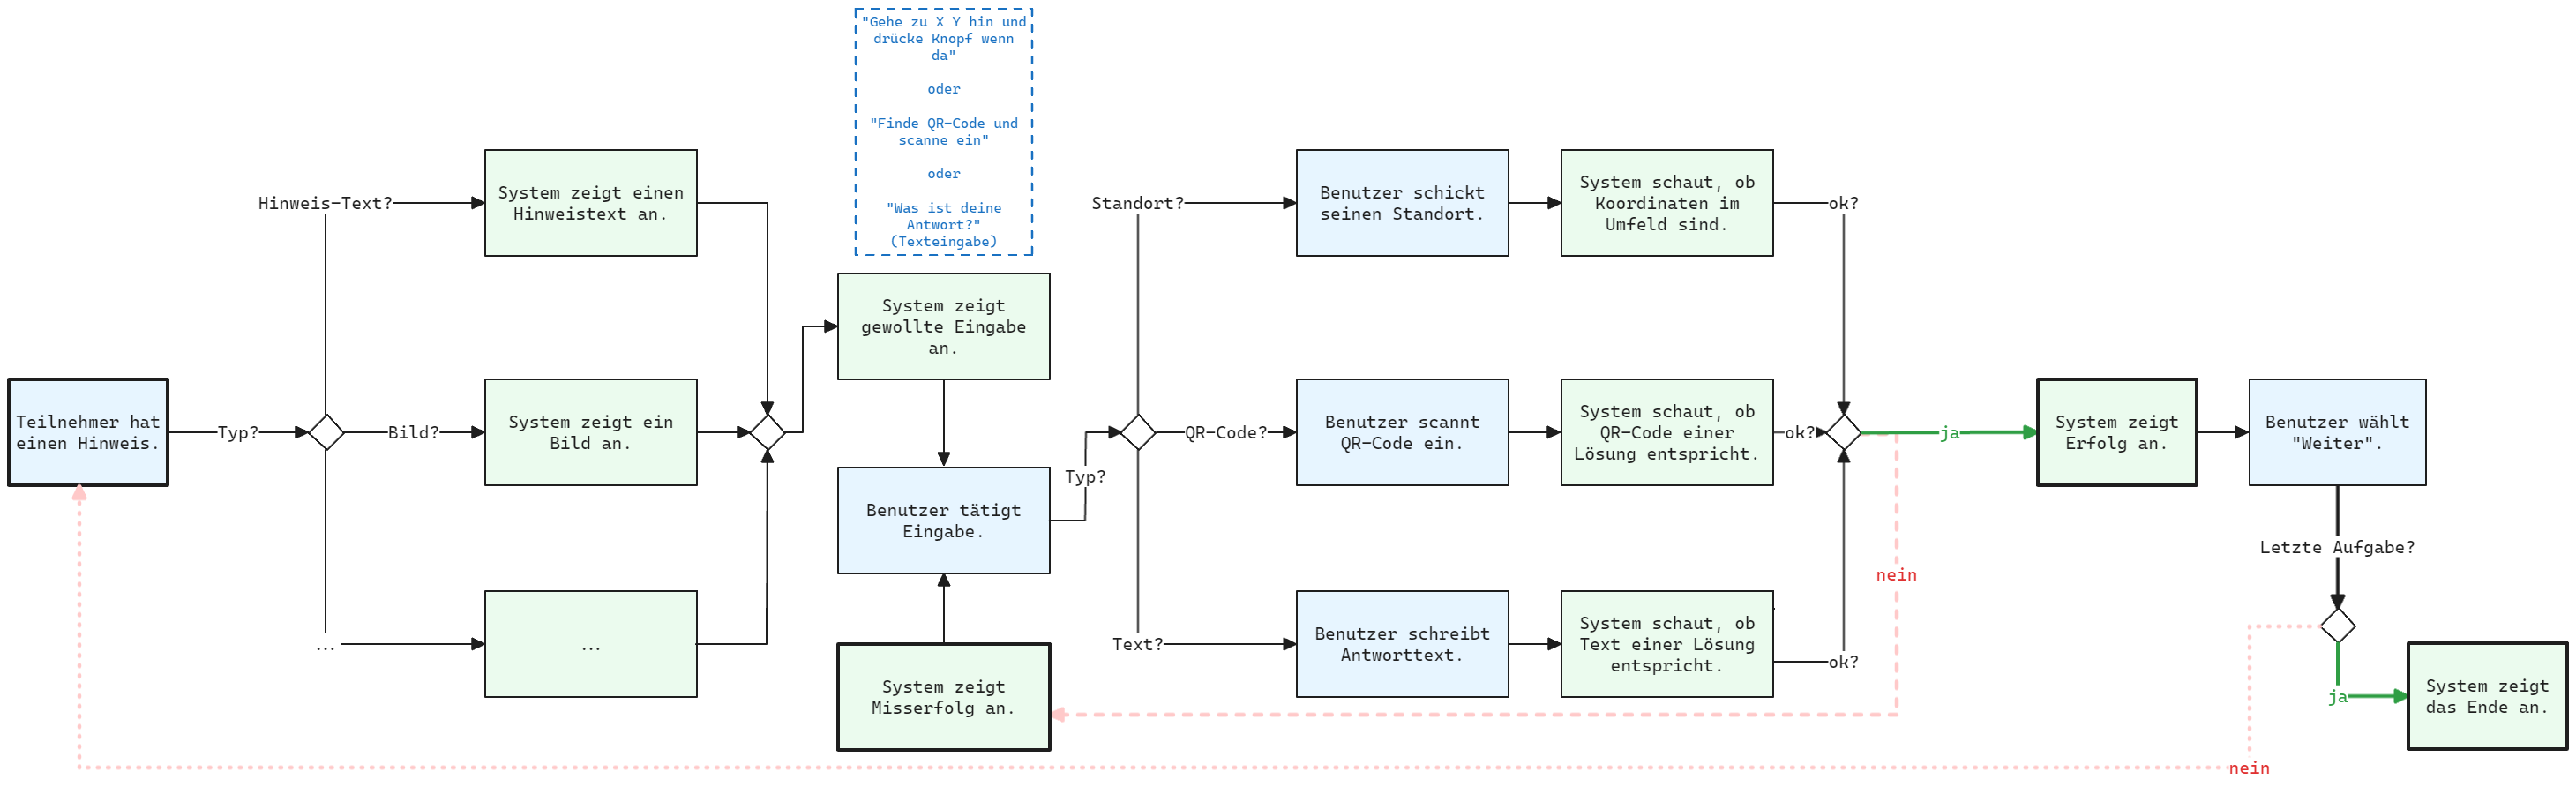
\includegraphics[width=\textwidth]{images/PrAr_Spielablauf.png}
  \caption{Skizze Spielablauf als UML-Programmablaufplan}
  \label{fig:hunt_game_spielablauf}
\end{figure}

Nachdem der Teilnehmer eine gültige Schnitzeljagd ausgewählt hat, beginnt der eigentliche Spielablauf. Zu Beginn wird dem Teilnehmer der aktuelle Hinweis präsentiert, der ihn zur nächsten Station oder Aufgabe führen soll. Die Hinweise sind in zwei Arten unterteilt: Text und Bild. Bei einem Texthinweis wird dem Teilnehmer ein beschreibender Text angezeigt, der Informationen oder Anweisungen zur nächsten Station enthält. Bei einem Bildhinweis wird stattdessen ein Bild angezeigt, das visuelle Hinweise oder Details enthält, die zur Lösung der Aufgabe beitragen.

Unter dem Hinweis befindet sich ein Button, über den der Teilnehmer seine Lösung einreichen kann. Es gibt drei verschiedene Lösungstypen, die je nach Aufgabe variieren:
\begin{itemize}
    \item \textbf{Textlösung}: Der Teilnehmer gibt seine Lösung in ein Textfeld ein. Dies kann z.B. ein gesuchtes Wort, ein Satz oder eine Zahlenkombination sein.

    \item \textbf{QR-Code}: Bei Aufgaben, die einen QR-Code erfordern, wird die Kamera des Gerätes aktiviert, um den QR-Code einzuscannen. Dieser QR-Code kann an verschiedenen Stellen versteckt sein und enthält die notwendigen Informationen oder Anweisungen, um zum nächsten Hinweis zu gelangen.

    \item \textbf{Location}: Wenn die Lösung in Form eines geographischen Ortes zur Verfügung gestellt werden soll, wird der Teilnehmer aufgefordert, den Zugriff auf den Ort zu erlauben. Der Browser ermittelt dann die aktuellen GPS-Koordinaten des Geräts und prüft, ob diese mit der erwarteten Lösung übereinstimmen.
\end{itemize}

Der Spielablauf wiederholt sich, bis alle Aufgaben gelöst sind. Bei den Lösungstypen Text und Ort erhält der Teilnehmer zusätzlich Hinweise, wenn seine Lösung nicht korrekt ist. Diese Hinweise besagen, dass die Lösung fast richtig ist, aber noch angepasst werden muss. Dies soll den Teilnehmer ermutigen und ihm die Möglichkeit geben, seine Antwort zu verbessern.






\chapter{Implementierung} \label{cha:implementierung}

\section{Entwickeln des Frontends}

\subsection{Aufbau der Web-Anwendungen}

\begin{figure}[H]
  \centering
  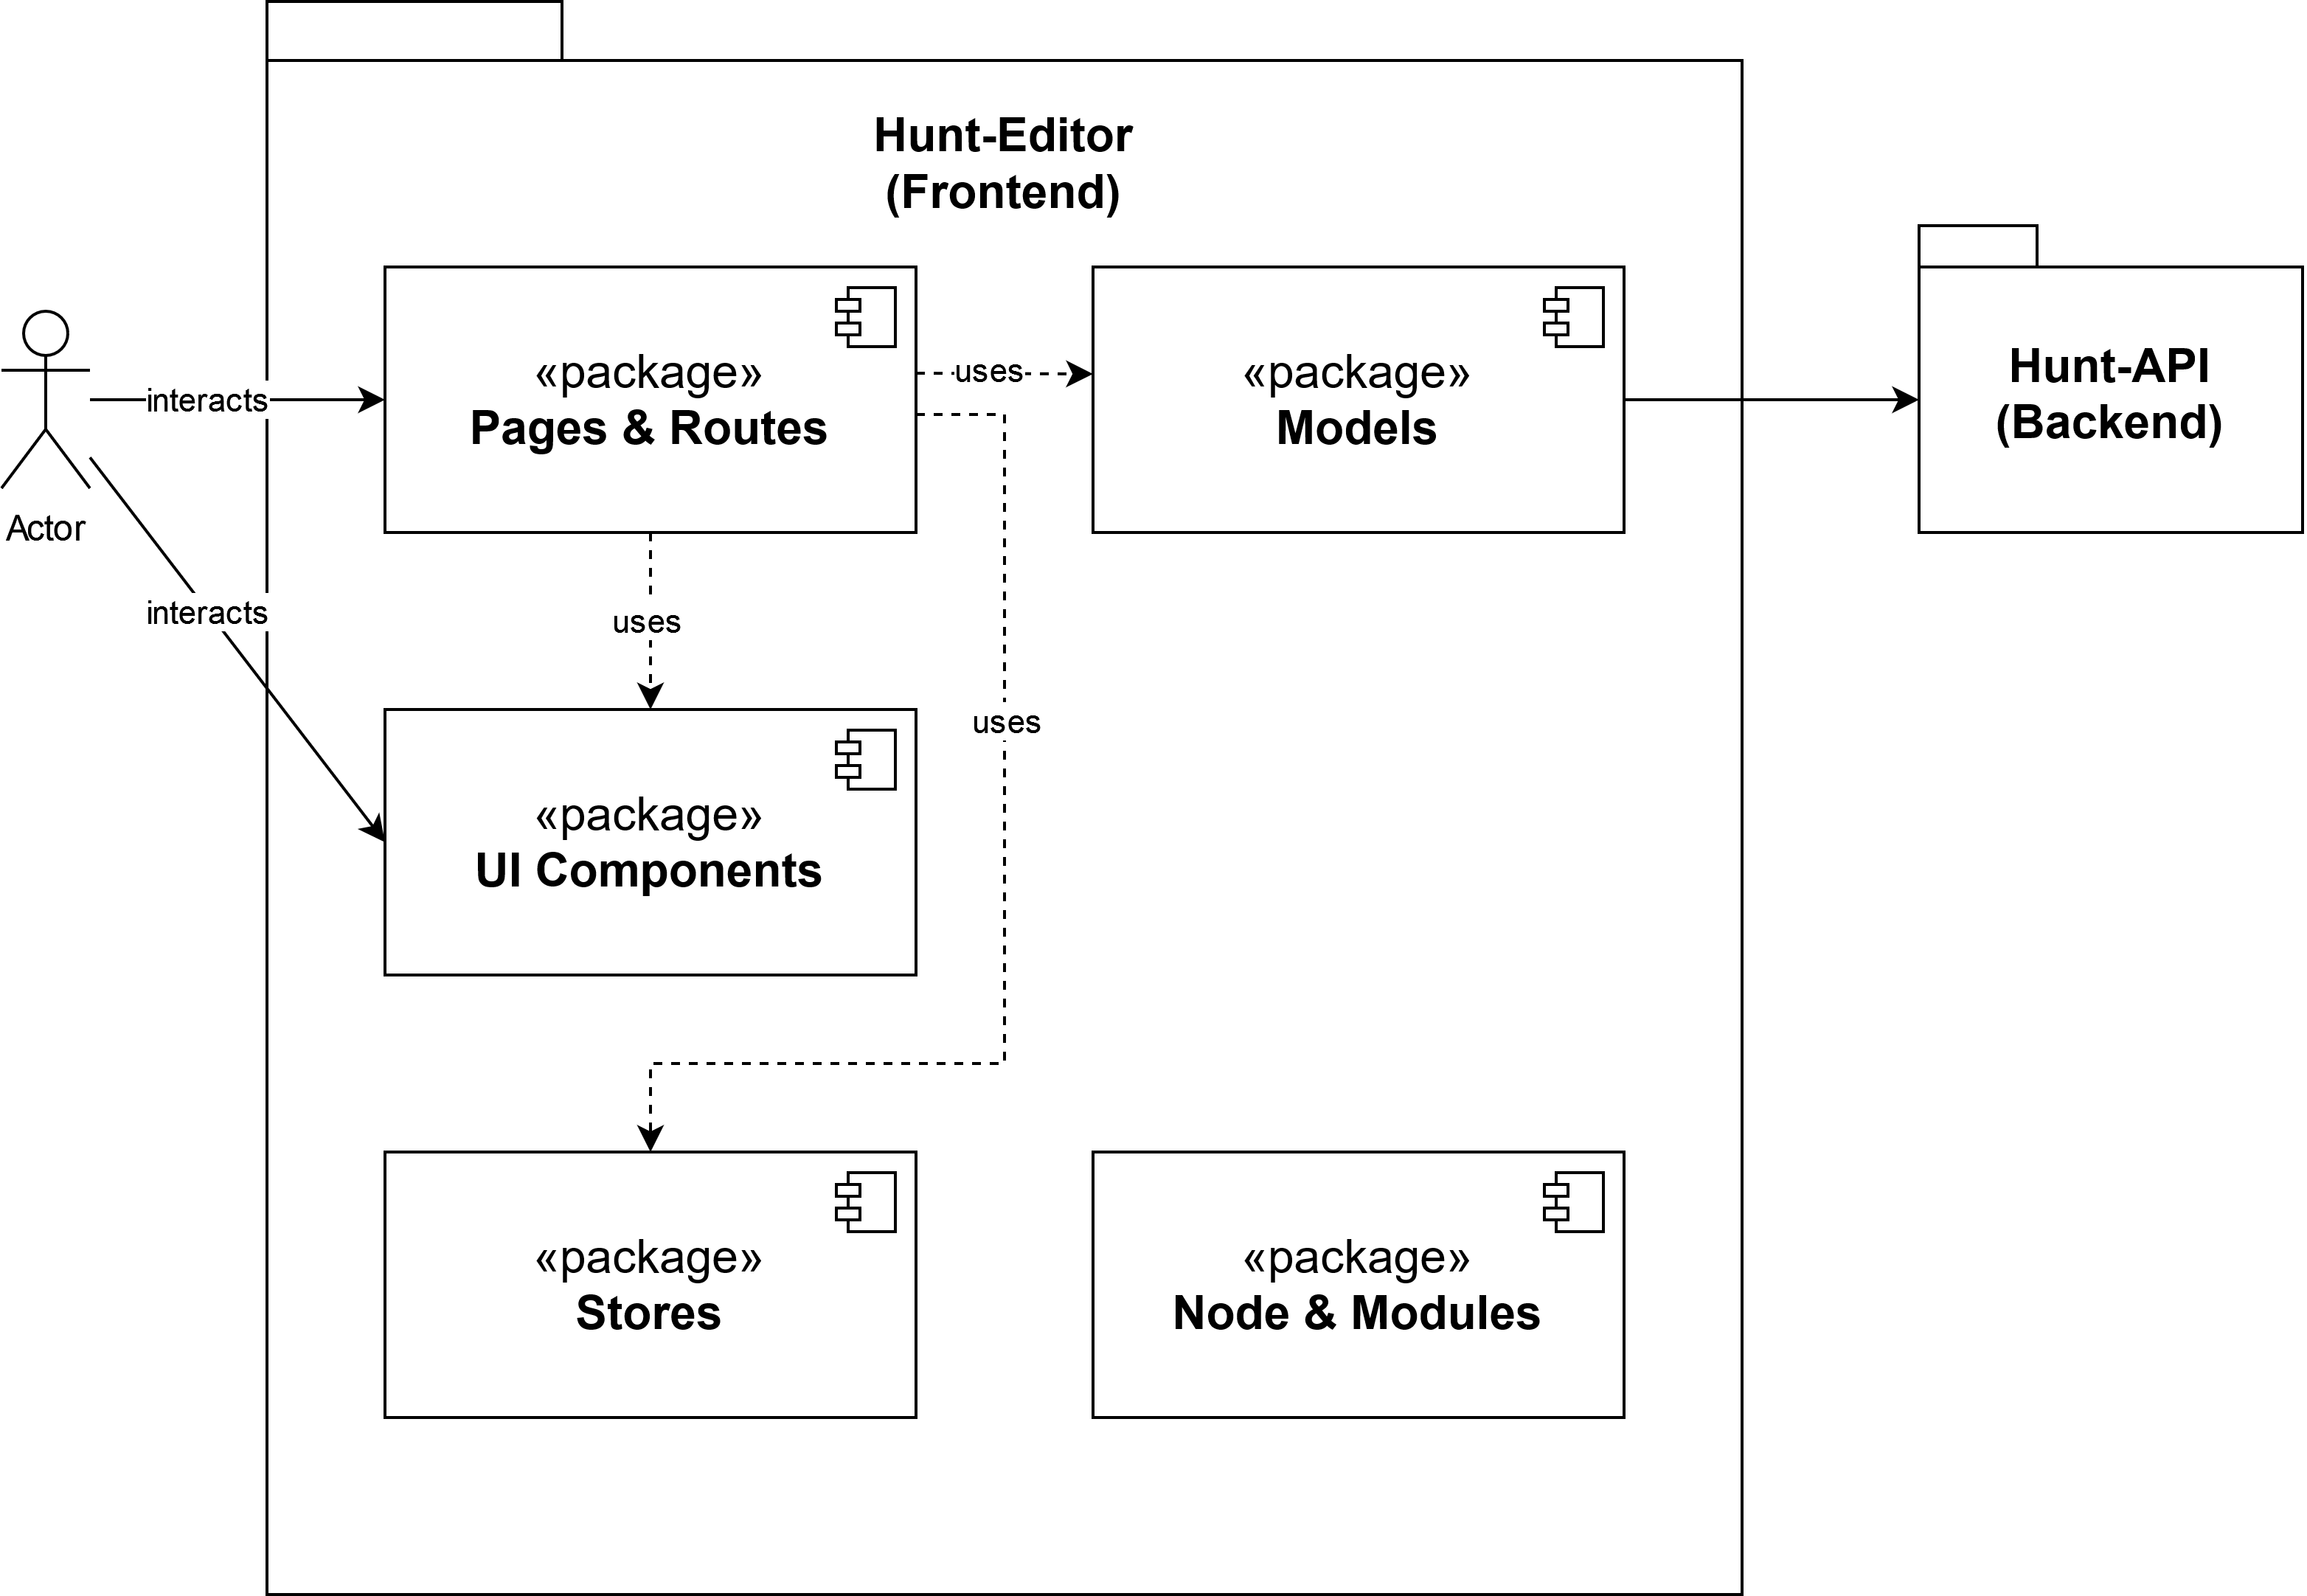
\includegraphics[width=1\textwidth]{images/PrAR-Loesung-Hunt-Editor-Components.png}
  \caption{UML-Diagramm Whitebox Frontend}
  \label{fig:whitebox-frontend}
\end{figure}

Abbildung \ref{fig:whitebox-frontend} veranschaulicht die grundlegenden Elemente, aus denen die Anwendungen bestehen. Für das Zwischenspeichern von anwendungsspezifischen Daten, wie beispielsweise Schnitzeljagd-Attribute (Titel, Beschreibung, Aufgaben) im Hunt-Editor oder der Teilnehmer-Token im Hunt-Game, werden Svelte Stores verwendet (vgl. Kapitel \ref{cha:grundlagen:swtech:svelte}).

\subsection{UI-Design}

Um die Anwendungen zu erstellen, wurde zunächst versucht, mit DaisyUI zu arbeiten. Da dies nicht das gewünschte Ergebnis geliefert hat, wurde zu Flowbite-Svelte gewechselt. Kapitel \ref{appendix:adr:daisy} begründet diese Entscheidung.

\subsection{Dynamic Routing}

In der Hunt-Editor Web-App wird das sogenannte \textit{Dynamic Routing} für das Editieren von Schnitzeljagden verwendet. Hierbei wird über die Route \textit{/edit/[huntId]} die \textit{id} der Schnitzeljagd dem Platzhalter \textit{[huntId]} in der Route eingefügt. Hierdurch kann Svelte über \textit{Load-Functions} dynamisch die Informationen einer Schnitzeljagd abrufen und anwendungsspezifisch speichern.

Das Dynamic Routing findet auch in der Participation Web-App verwendung. Über die Route \textit{/participation/[huntId]} wird in einer Svelte \textit{Load-Function} ebenso Titel und Beschreibung einer Schnitzeljagd geladen.

Im Anhang \ref{appendix:code:dynamicrouting} wird die Implementierung des Dynamic Routings näher verdeutlicht.

\subsection{Walkthrough der Web-Anwendungen}

Im Anhang \ref{appendix:code:walkthrough} wird zu den jeweiligen Web-Anwendungen ein Walkthrough geliefert.

\section{Entwickeln einer AR-Anwendung mit Unity und AR-Foundation} \label{cha:implementierung:unityardev}

Im Folgenden wird der Entwicklungsprozess für das Implementieren eines AR-Image-Trackers mithilfe des AR-Foundation Frameworks von Unity beschrieben. Im Anschluss erfolgt eine Erläuterung der Gründe, welche dazu führten, dass dieser Ansatz für das Projekt als nicht länger geeignet erachtet wurde.

Für die Entwicklung mit Unity wird die Installation des Unity-Hubs sowie einer unterstützten Version des Unity-Editor vorausgesetzt. Die im Projekt entwickelte Anwendung wurde mit der Editor-Version \textit{2022.3.20f1} erstellt.

\subsection{Anlegen einer Reference-Image-Library}

Nach der Erstellung eines AR-Unity-Projekts gemäß \autocite{Unity2024:ProjectSetup} angelegt wurde und der erfolgreichen Integration des erforderlichen Frameworks, stehen im Editor verschiedene Funktionen des AR-Foundation-Frameworks zur Verfügung.

Zunächst soll eine \textit{Reference-Image-Library} erstellt werden. Abbildung \ref{fig:implementierung:unity:AR-Create-Img-Lib} markiert die grundlegenden Schritte hierfür.

\begin{figure}[H]
    \centering
    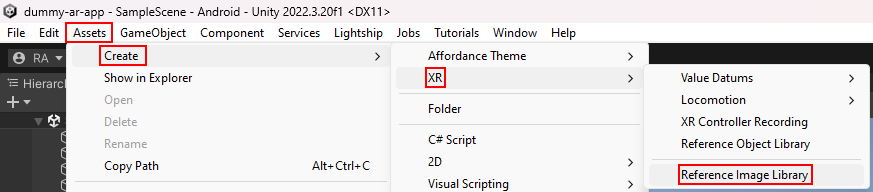
\includegraphics[width=\textwidth]{images/PrAr_UnityAR-Create-Img-Lib.png}
    \caption{Bildschirmabschnitt für das Erstellen einer Reference-Image-Library}
    \label{fig:implementierung:unity:AR-Create-Img-Lib}
\end{figure}

In der geöffneten Szene in Abbildung \ref{fig:implementierung:unity:AR-See-Img-Lib} sollte nun ein leeres Reference-Image-Library Objekt existieren.

\begin{figure}[H]
    \centering
    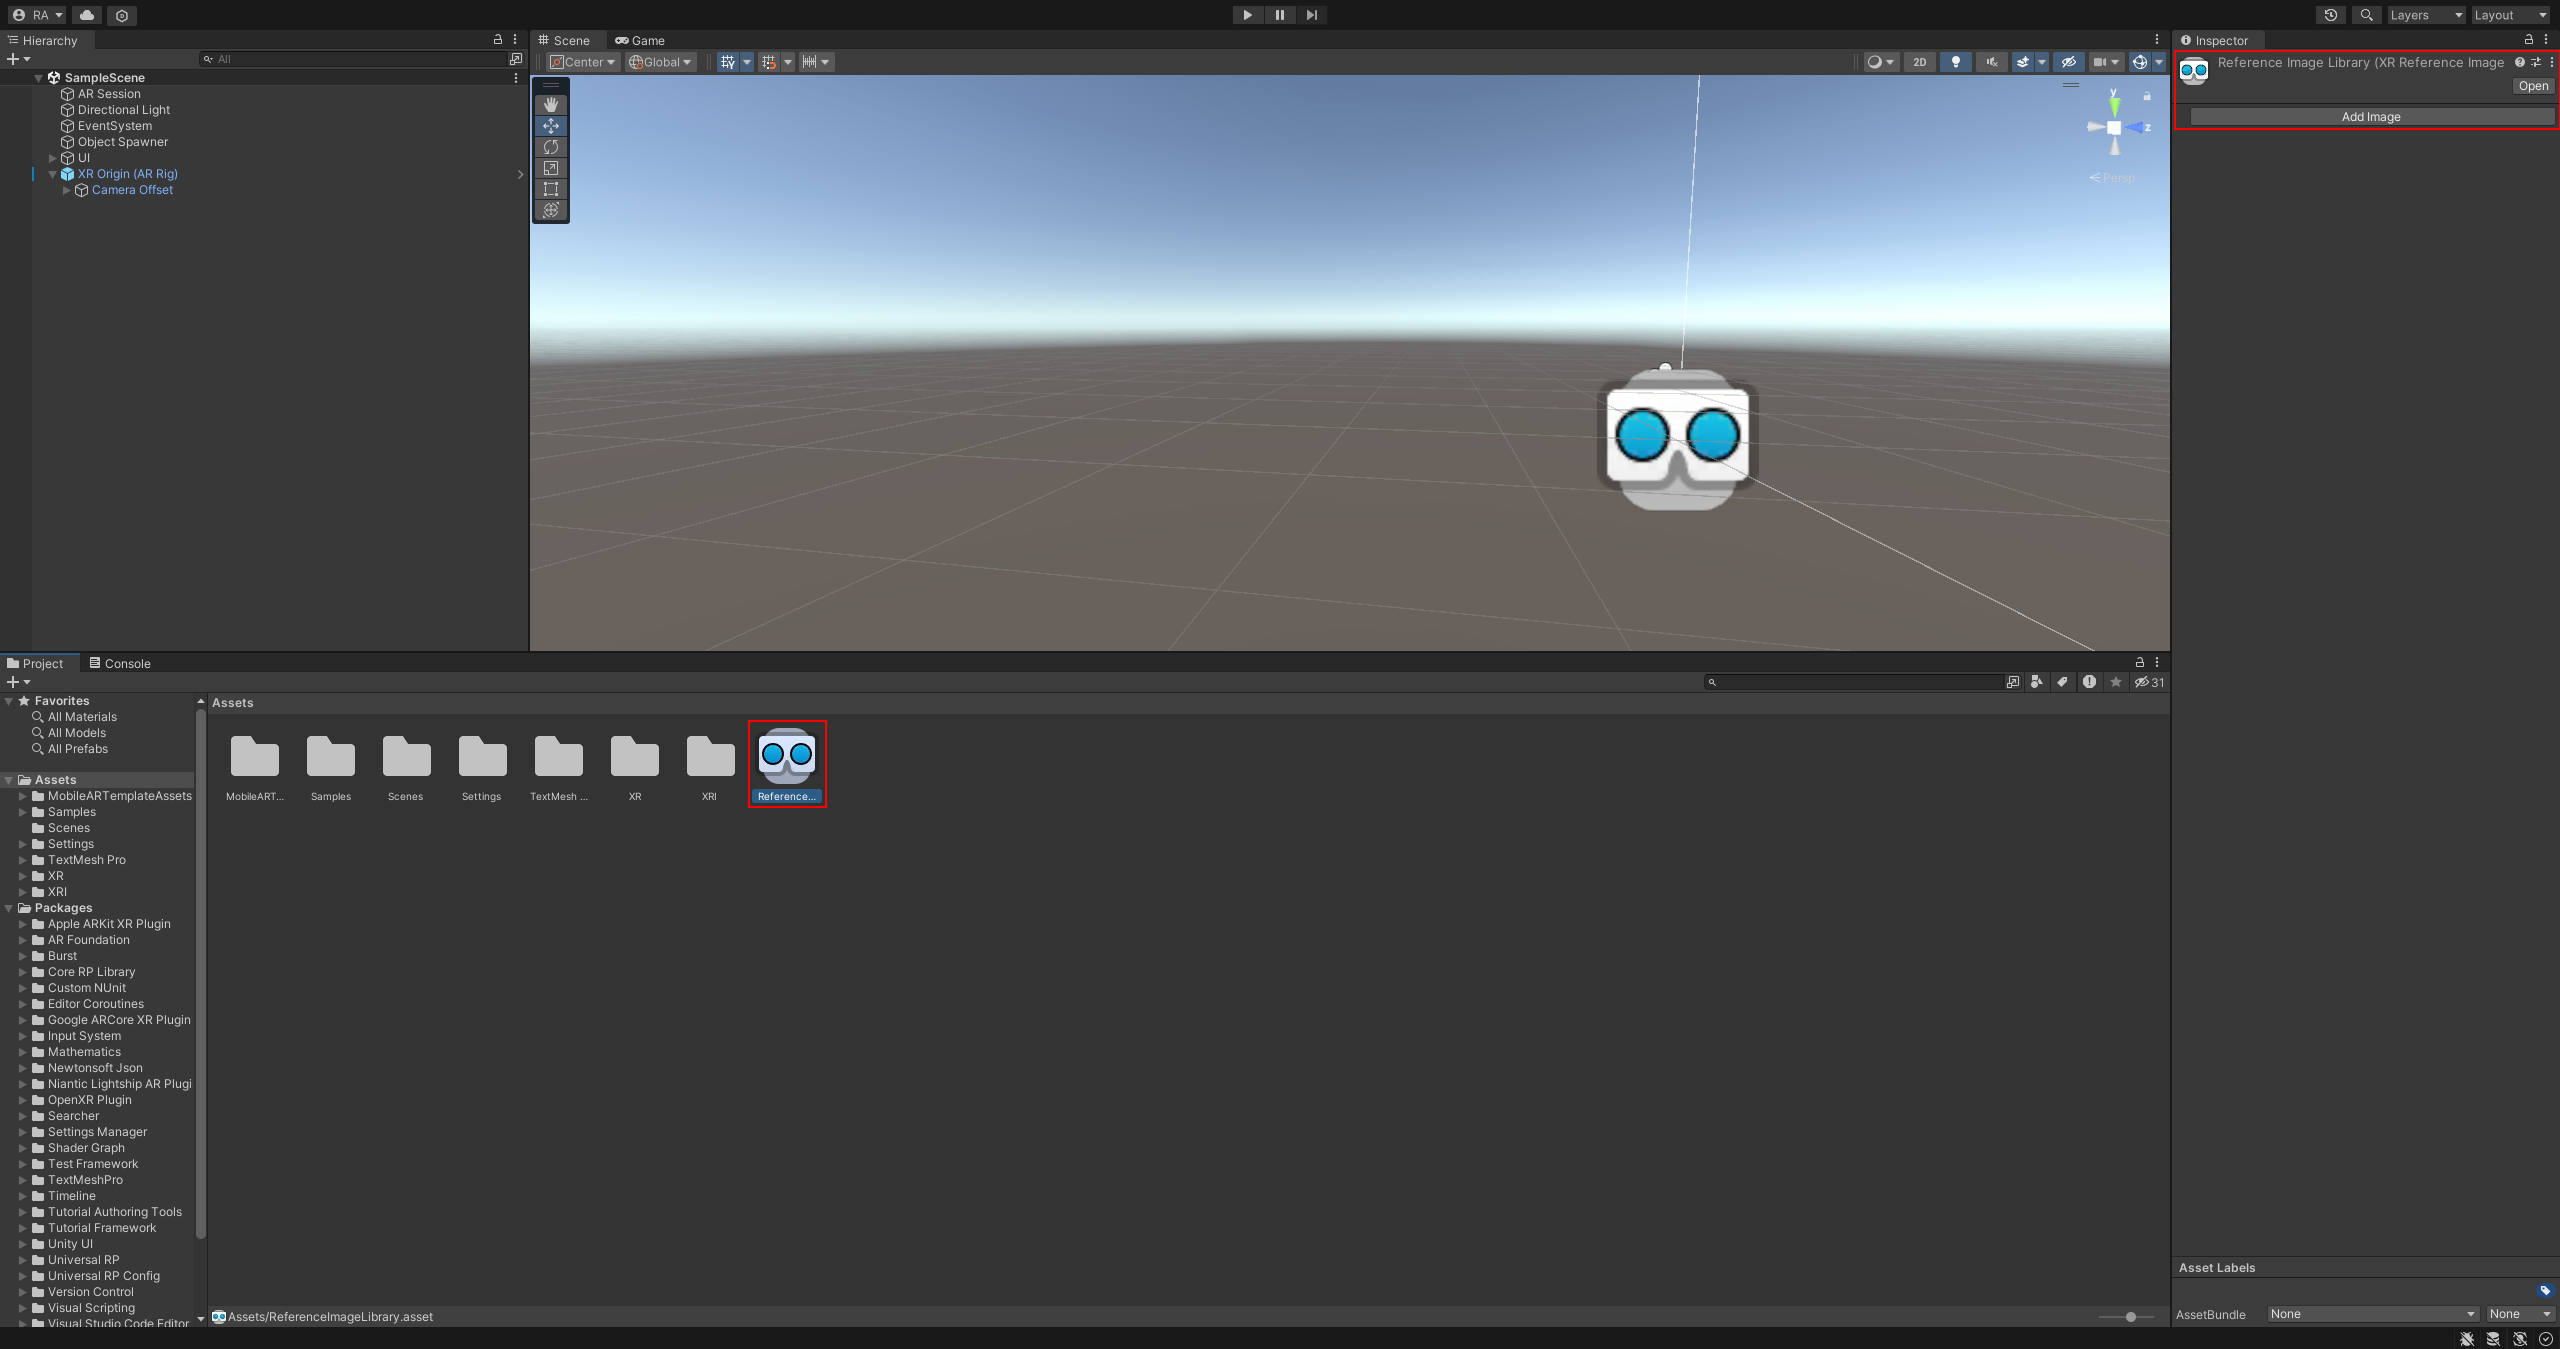
\includegraphics[width=\textwidth]{images/PrAr_UnityAR-See-Img-lib.png}
    \caption{Bildschirmabschnitt Reference-Image-Library Objekt im Editor}
    \label{fig:implementierung:unity:AR-See-Img-Lib}
\end{figure}

Die Reference-Image-Library wird benötigt, um bereits vor der Laufzeit bereits Referenzbilder (\textit{Reference-Images}) oder Objekte zu sammeln, die von einem AR-Tracker wie etwa der Komponente \textit{XRImageTrackingSubsystem} erkannt werden können.

\subsection{Anlegen eines AR-Tracked-Image-Managers}

Die Komponente \textit{AR Tracked Image Manager} generiert \textit{Game-Objects} für jedes gefundene Bild innerhalb des Viewports des Benutzers. Die Fähigkeit, Bilder zu finden, setzt voraus, dass die Komponente \textit{Reference-Images} kennt, die in der \textit{Reference-Image-Library} gespeichert sind.

Das Einbinden erfolgt durch die Anbindung eines Skripts an die \textit{XR-Origin} Komponente und die entsprechende Einbindung der \textit{Reference-Image-Library} per Drag-and-Drop. Dies aktiviert das Tracken von Bildern im AR-Raum.

\begin{figure}[H]
    \centering
    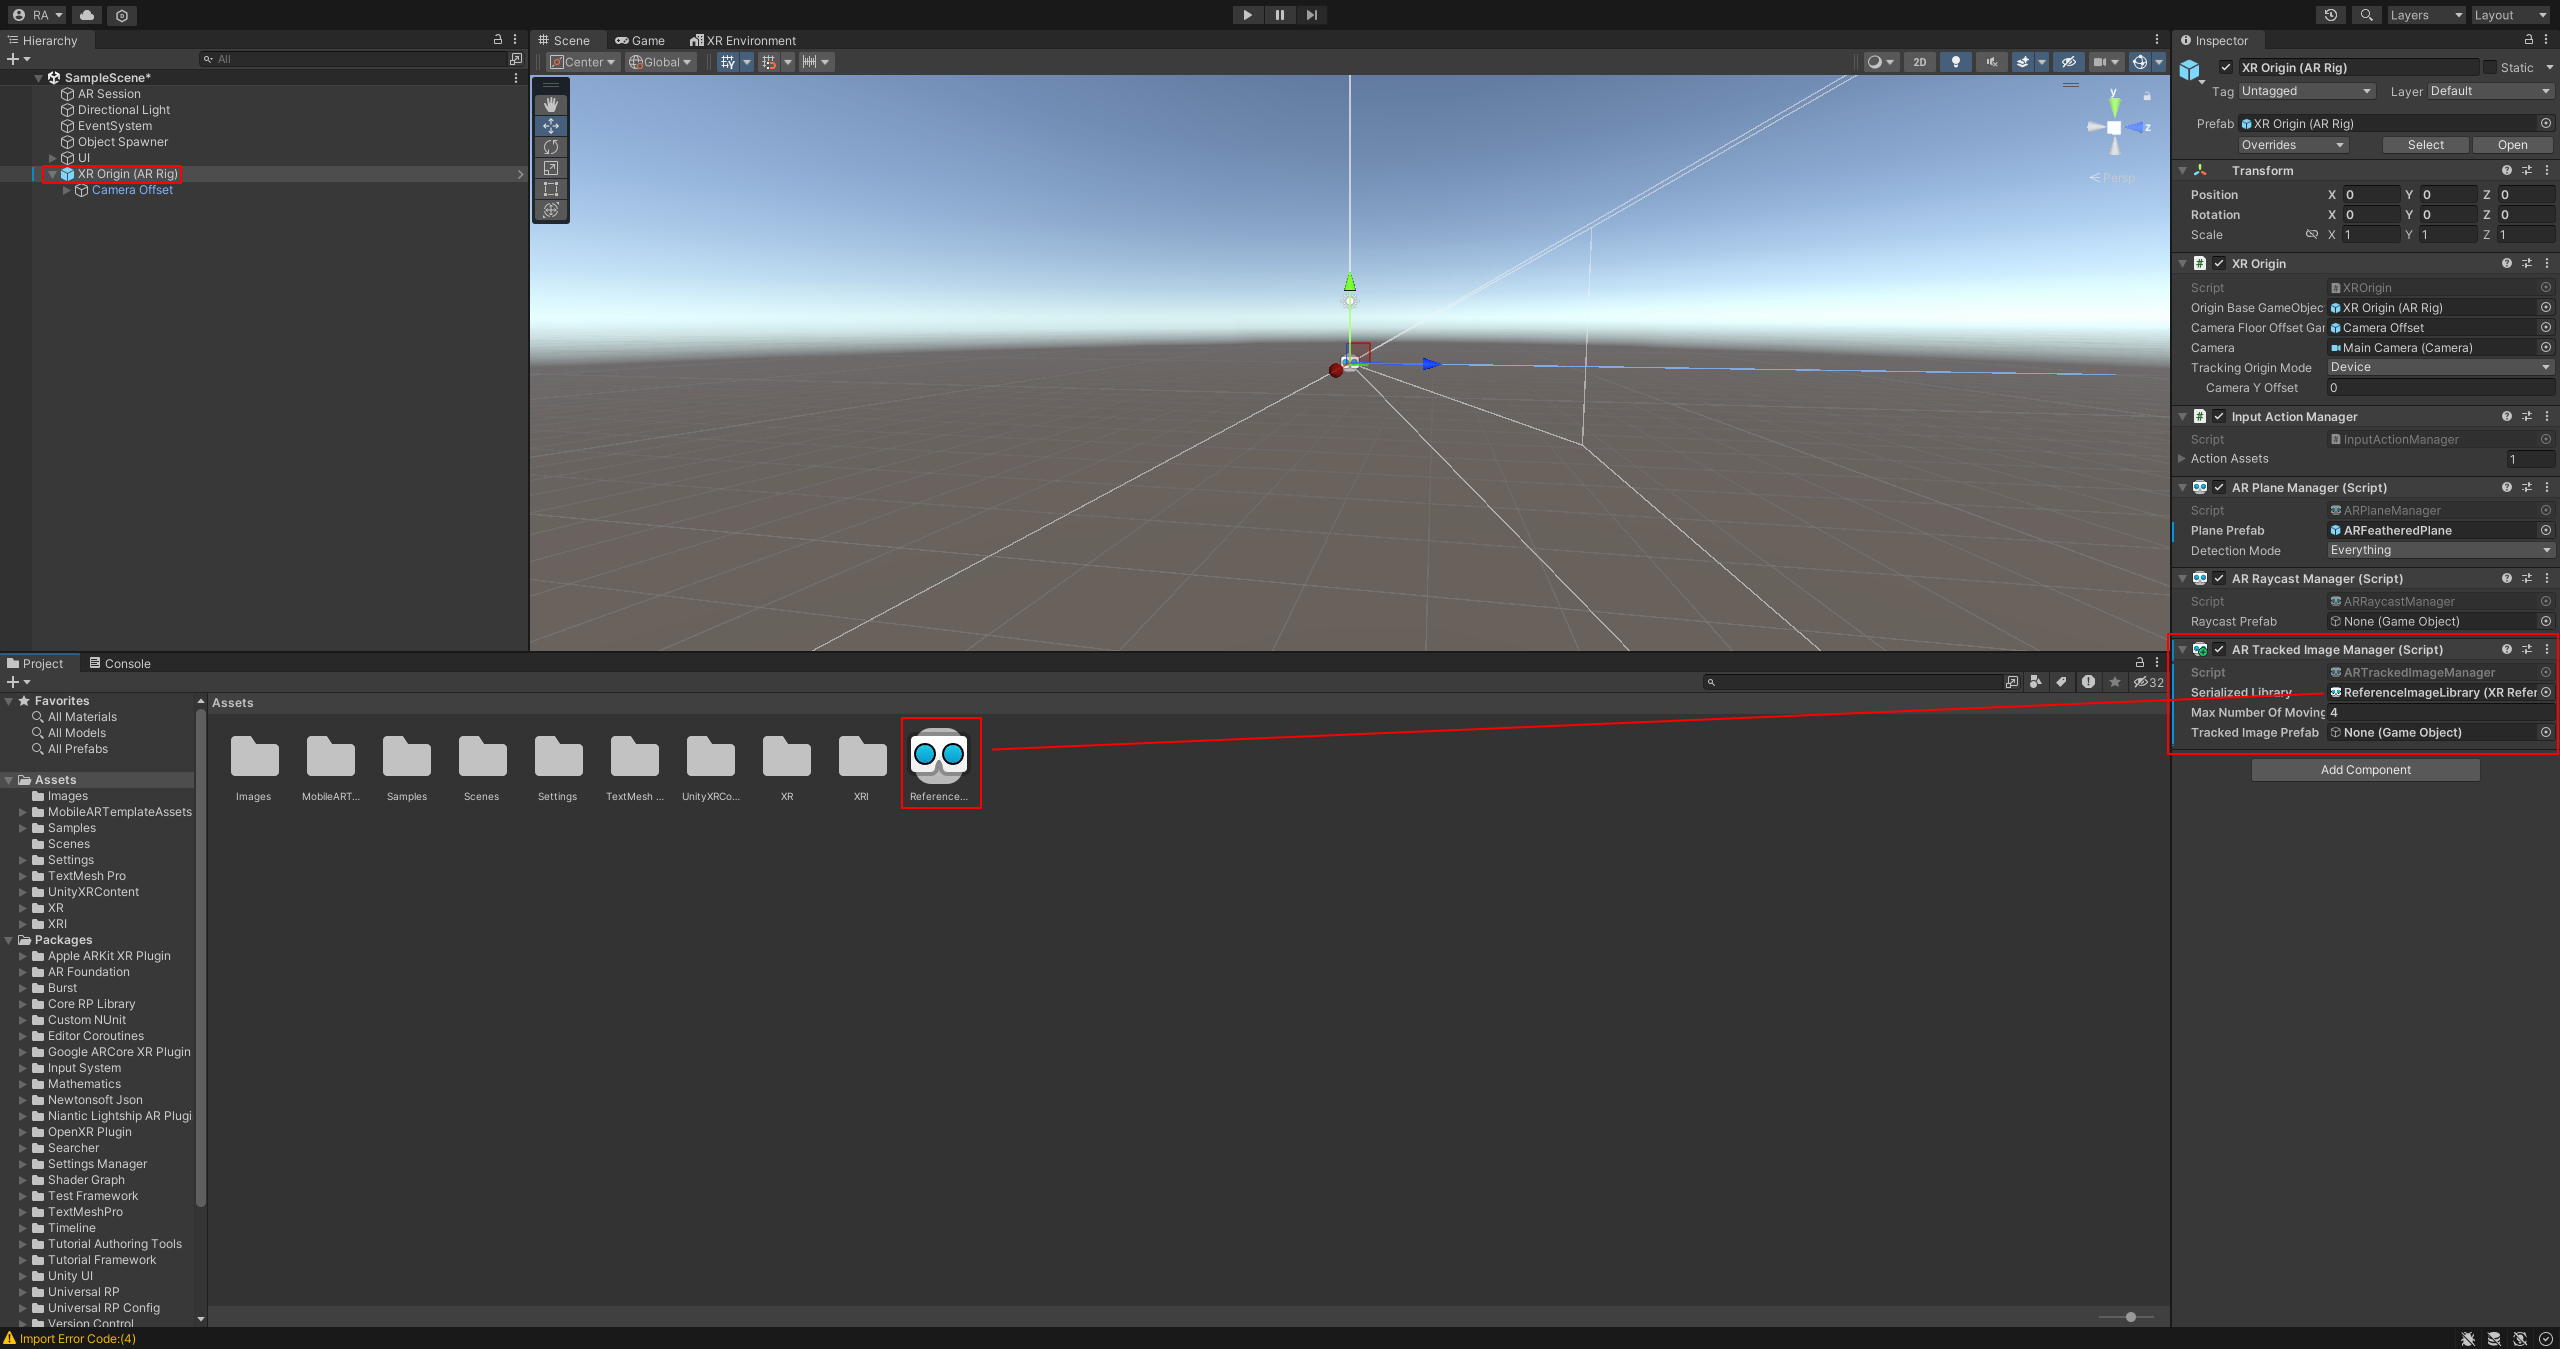
\includegraphics[width=\textwidth]{images/PrAr_UnityAR-Create-Img-Mngr.png}
    \caption{Bildschirmabschnitt für das Erstellen eines AR-Tracked-Image-Managers}
    \label{fig:implementierung:unity:AR-Create-Img-Mngr}
\end{figure}

\subsection{QR-Code-Daten aus einem Referenz-Bild lesen}

Die Erkennung eines QR-Codes etzt voraus, dass dieser zuvor in der \textit{Reference-Image-Library} angelegt wurde. Der QR-Code kann dadurch als Textur eingelesen und über einen QR-Code-Konverter wie \textit{ZXing} als Text konvertiert werden. Abbildung \ref{fig:implementierung:unity:AR-Read-Qr-Img} zeigt das erfolgreiche Umkonvertieren eines QR-Codes im AR-Raum.

\begin{figure}[H]
    \centering
    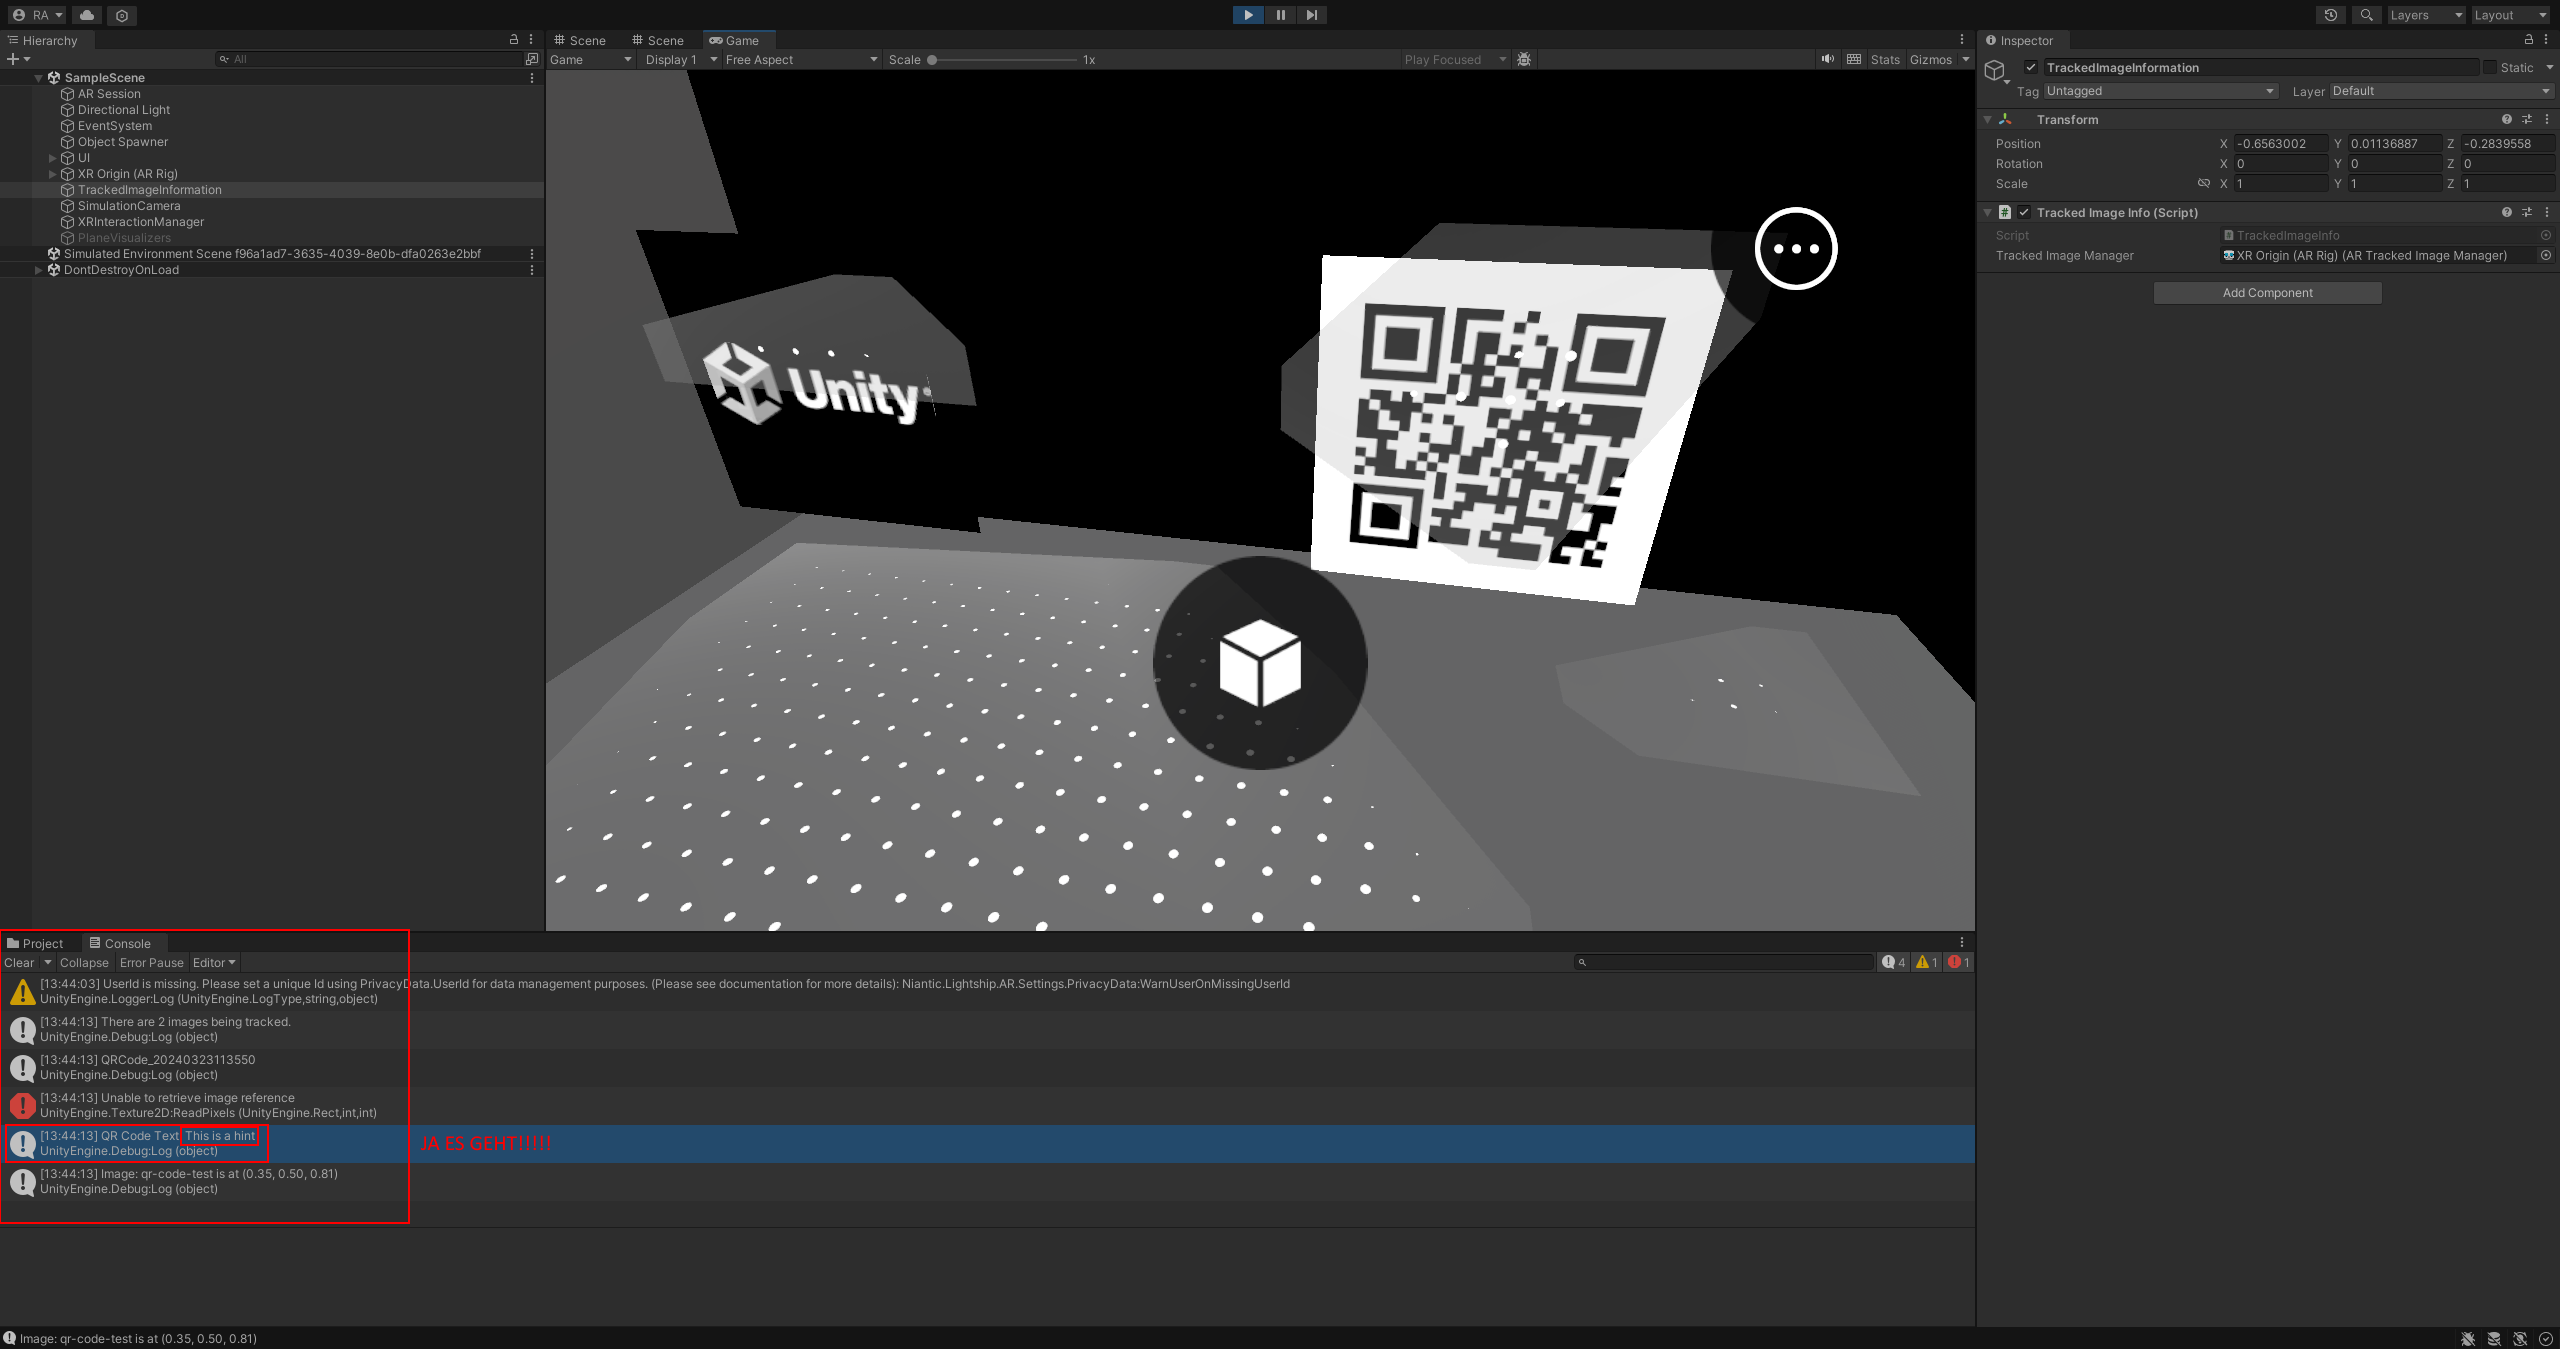
\includegraphics[width=\textwidth]{images/PrAr_UnityAR-Read-Qr-Img.png}
    \caption{Bildschirmabschnitt für das Lesen eines QR-Codes}
    \label{fig:implementierung:unity:AR-Read-Qr-Img}
\end{figure}

\subsection{Erfahrung mit Unity und AR-Foundation}

Leider führte das in Kapitel \ref{cha:implementierung:unityardev} beschriebene Vorgehen nicht zum gewünschten Resultat.

Ein Hinweistext oder -bild an der Position des QR-Codes zu platzieren, könnte theoretisch funktionieren, wie in Abbildung \ref{fig:implementierung:unity:AR-Read-Qr-Img} bereits dargestellt wird. Allerdings stellt die mangelnde Flexibilität der Reference-Image-Library ein erhebliches Hindernis für eine funktionierende Implementierung dar.

Um das beschriebene Problem zu vermeiden, wäre es erforderlich, dass die Anwendung beim Start alle im System vorhandenen QR-Codes und ihre entsprechenden Lösungen über das Backend abruft. Dies würde jedoch bei einer großen Anzahl von QR-Codes zu einer suboptimalen Benutzererfahrung führen, da die Anwendung erheblich verzögert wäre. Zusätzlich verursacht das Laden mehrerer QR-Codes einen hohen Speicheraufwand.

Des Weiteren werden die Lösungen vor dem Erhalt eines ersten Hinweises auf dem Gerät des Teilnehmers geladen. Dies könnte zur Konsequenz haben, dass manche Lösungen aus den geladenen Bildern extrahiert werden können, wodurch das Konzept der Schnitzeljagd umgangen wird.

Die genannten Herausforderungen verdeutlichen, dass Unity und das AR Foundation Framework in diesem Kontext keine optimale Lösung darstellen. Die genannten Einschränkungen erschweren die Entwicklung einer flexiblen, effizienten und sicheren Anwendung, die den Anforderungen einer Schnitzeljagd entspricht. Daher ist es empfehlenswert, alternative Technologien oder Ansätze zu berücksichtigen, die eine bessere Anpassungsfähigkeit und Sicherheit bieten.

Die Entscheidung, Unity als ganzes nicht für das Schnitzeljagd-Spiel zu verwenden, wird zudem in folgenden Aspekten begründet.

\subsubsection{Entwicklungsumgebung und Tooling}
\label{subsubsec:implementierung:unity:unityeditor}

Die Entwicklungsumgebung und der Entwicklungsprozess, die für die Erstellung einer Anwendung in Unity erforderlich sind, weisen erhebliche Nachteile auf. Das Tooling von Unity ist oft unhandlich und ineffizient. Häufig auftretende Probleme müssen durch Neustarts des Unity-Hubs oder des Unity-Editors gelöst werden. Diese häufigen Unterbrechungen führen zu einem erheblichen Zeitverlust, der den Entwicklungsprozess stark behindert.

Ein weiteres Problem ist die resultierende Größe der Anwendung nach dem Build. Die Unity-Engine erzeugt sehr große Dateien, selbst wenn nur grundlegende Funktionen verwendet werden. Eine Optimierung auf das Nötigste ist kaum möglich, was die Anwendung unnötig aufbläht und somit unpraktisch für mobile Geräte macht.

\subsubsection{Anpassung auf Projektanforderungen}

AR Foundation, die AR-Entwicklungsplattform von Unity, bietet für unsere Schnitzeljagd-Anwendung keine entscheidenden Vorteile. Unsere Anwendung konzentriert sich hauptsächlich auf die Darstellung von Texten und Bildern sowie das Scannen von QR-Codes, was keine umfassende AR-Funktionalität erfordert. Eine einfache und ressourcenschonende Lösung wäre hier weitaus effizienter.

\subsubsection{Lizensierung und Business}

In den vergangenen Monaten hat das Unternehmen \textit{Unity Technologies}, welches hinter Unity steht, erheblich an Reputation verloren. Dies ist auf umstrittene Änderungen der Lizenzbedingungen und Preismodelle zurückzuführen. Diese Änderungen haben bei Entwicklern für Unmut gesorgt und das Vertrauen in das Unternehmen erschüttert. \autocite{Unity2024:PriceChange}

Die negativen Schlagzeilen und die Unsicherheit über zukünftige Geschäftsstrategien machen Unity zu einer risikobehafteten Wahl für langfristige Projekte.

\subsection{Alternativen}

\subsubsection{Vuforia}

Vuforia ist eine AR Plattform, die, ähnlich wie AR Foundation, ermöglicht, Augmented Reality in mobilen Anwendungen zu integrieren. Vuforia bietet verschiedene Funktionen wie Bilderkennung, Objektverfolgung und die Möglichkeit, 3D-Modelle in reale Umgebungen einzubetten. Diese Plattform ist besonders bekannt für ihre zuverlässige Erkennung und Nachverfolgung von Bildern und Objekten, was sie zu einer beliebten Wahl für AR-Entwickler macht \autocite{Vuforia2024:Features}.

Trotz dieser Fähigkeiten gibt es mehrere Gründe, warum Vuforia für das aktuelle Projekt nicht die optimale Wahl ist:

\begin{itemize}
    \item \textbf{Abhängigkeit vom Unity-Editor}: Vuforia ist stark in den Unity-Editor integriert. Dies bedeutet, dass Entwickler, die Vuforia nutzen, auch die Unity-Plattform verwenden müssen, was bereits in Kapitel \ref{subsubsec:implementierung:unity:unityeditor} als problematisch identifiziert wurde. Die Nachteile des Unity-Editors würden somit auch bei der Verwendung von Vuforia bestehen bleiben.
    \item \textbf{Alternativer Entwicklungsaufwand}: Eine Alternative zur Verwendung von Unity wäre die Integration von Vuforia in eine Android-App über Android Studio. Dies würde jedoch zusätzliche Lernkurven und Einarbeitungszeit erfordern, da ein neues Toolset gemeistert werden müsste. Für ein Projekt, das hauptsächlich auf Webtechnologien basiert, würde dies einen erheblichen zusätzlichen Aufwand bedeuten.
    \item \textbf{Kosten}: Vuforia hat eine Lizenzgebührstruktur, die je nach Nutzung und Funktionalitäten variieren kann. Die Preise können für kleinere Projekte oder akademische Arbeiten unerschwinglich sein \autocite{Vuforia2024:Pricing}.
\end{itemize}

Insgesamt bieten die Nachteile von Vuforia, insbesondere in Verbindung mit den bereits erwähnten Problemen von Unity, eine unzureichende Grundlage für die Umsetzung des Projekts. Die Kombination aus technischen Herausforderungen, zusätzlichem Entwicklungsaufwand und potenziellen Kosten macht Vuforia zu einer weniger idealen Wahl im Vergleich zu alternativen Ansätzen wie WebAR, die für die spezifischen Anforderungen des Projekts besser geeignet sind.


\subsubsection{WebAR}

Eine vielversprechende Alternative zur nativen AR-Entwicklung mit Unity ist WebAR. WebAR ermöglicht AR-Erlebnisse direkt im Webbrowser ohne die Notwendigkeit einer separaten App-Installation. Dies bietet mehrere Vorteile:

\begin{itemize}
    \item \textbf{Zugänglichkeit}: WebAR ist auf jedem modernen Webbrowser verfügbar, was die Zugänglichkeit für Benutzer erleichtert und die Notwendigkeit, eine spezielle App herunterzuladen, beseitigt. Dies kann die Benutzerfreundlichkeit und die Reichweite der Anwendung erhöhen.
    \item \textbf{Einfachere Entwicklung}: WebAR nutzt Web-Technologien wie JavaScript und WebGL, die für viele Entwickler vertrauter und zugänglicher sind als die speziellen Tools und Skripte von Unity. Die Entwicklung kann daher schneller und einfacher sein, besonders wenn bereits Erfahrung mit Web-Technologien besteht.
    \item \textbf{Kosteneffizienz}: Da WebAR keine zusätzlichen Lizenzgebühren oder Laufzeitgebühren erfordert, ist es eine kostengünstigere Lösung.
\end{itemize}

\subsubsection{Schlussfolgerung}

Falls die Schnitzeljagd Anwendung in Zukunft AR-Funktionen beinhalten soll, stellt WebAR die effizienteste und kostengünstigste Lösung dar. Es bietet eine einfache und zugängliche Möglichkeit, grundlegende AR-Funktionen bereitzustellen, ohne die Notwendigkeit einer komplexen Entwicklungsumgebung. Vuforia und Unity bieten erweiterte Funktionen, die für diese Anwendung nicht erforderlich sind und könnten daher überdimensioniert sein.

%------------------------------------%

\section{Algorithmen zur Hinweisbestimmung für Nutzerlösungen}

Zwei Algorithmen wurden implementiert, um dem Benutzer Hinweise zu geben, dass eine von ihm eingegebene Lösung nahezu richtig ist. Diese Algorithmen helfen, den Grad der Übereinstimmung zwischen der vom Benutzer angegebenen Lösung und der tatsächlich gesuchten Antwort zu bestimmen.

\subsection{Haversine-Algorithmus zur Bestimmung geografischer Distanzen}

Einer der Algorithmen kommt zum Einsatz, wenn die Lösung einen geografischen Ort umfasst, der durch Breiten- und Längengrade (Latitude und Longitude) definiert ist. Hier wird die Haversine-Formel verwendet, um die Entfernung zwischen den beiden Punkten zu berechnen.

Die Haversine-Formel erweist sich als überaus nützlich bei der Ermittlung der kürzesten Entfernung über die Erdoberfläche, da sie die Krümmung der Erde adäquat berücksichtigt. Diese Berechnung ist von essenzieller Bedeutung, um zu bestimmen, wie nahe ein Nutzer mit seiner Antwort an der korrekten Position liegt.

Der folgende C\#-Code zeigt die Implementierung des Haversine-Algorithmus:

\begin{lstlisting}[language=c, caption={Code Ausschnitt zum Haversine Algorithmus in C\#}]
public static double Haversine(double lat1, double lon1, double lat2, double lon2)
{
    // Convert degrees to radians
    double dLat = ToRadians(lat2 - lat1);
    double dLon = ToRadians(lon2 - lon1);

    lat1 = ToRadians(lat1);
    lat2 = ToRadians(lat2);

    // Haversine formula
    double a = Math.Sin(dLat / 2) * Math.Sin(dLat / 2) +
               Math.Sin(dLon / 2) * Math.Sin(dLon / 2) * Math.Cos(lat1) * Math.Cos(lat2);
    double c = 2 * Math.Atan2(Math.Sqrt(a), Math.Sqrt(1 - a));

    // Distance in meters
    return RADIUS_OF_EARTH_METERS * c;
}

private static double ToRadians(double angleInDegrees)
{
    return angleInDegrees * Math.PI / 180.0;
}
\end{lstlisting}

In diesem Algorithmus wird zunächst die Differenz zwischen den Längen- und Breitengraden der beiden Punkte berechnet und in Radianten umgewandelt. Anschließend wird die Haversine-Formel angewendet, um den Anteil des großen Kreises (die kürzeste Strecke zwischen zwei Punkten auf der Oberfläche einer Kugel) zu berechnen, den der Abstand zwischen den Punkten darstellt. Dieser Anteil wird dann mit dem Radius der Erde multipliziert, um die tatsächliche Entfernung in Metern zu erhalten.

Die Berechnung ermöglicht dem System die Bestimmung der Distanz zwischen dem vom Nutzer angegebenen Ort und der korrekten Position. Bei einem geringen Abstand liefert das System ein Feedback, das darauf hinweist, dass die Lösung nahe dran ist.

\subsubsection{Anwendungsbeispiel des Haversine-Algorithmus}

Im folgenden wird der Harvesine-Algorithmus zum Bestimmen der Distanz des Benutzers zur Lösung verwendet.

\begin{figure}[H]
    \centering
    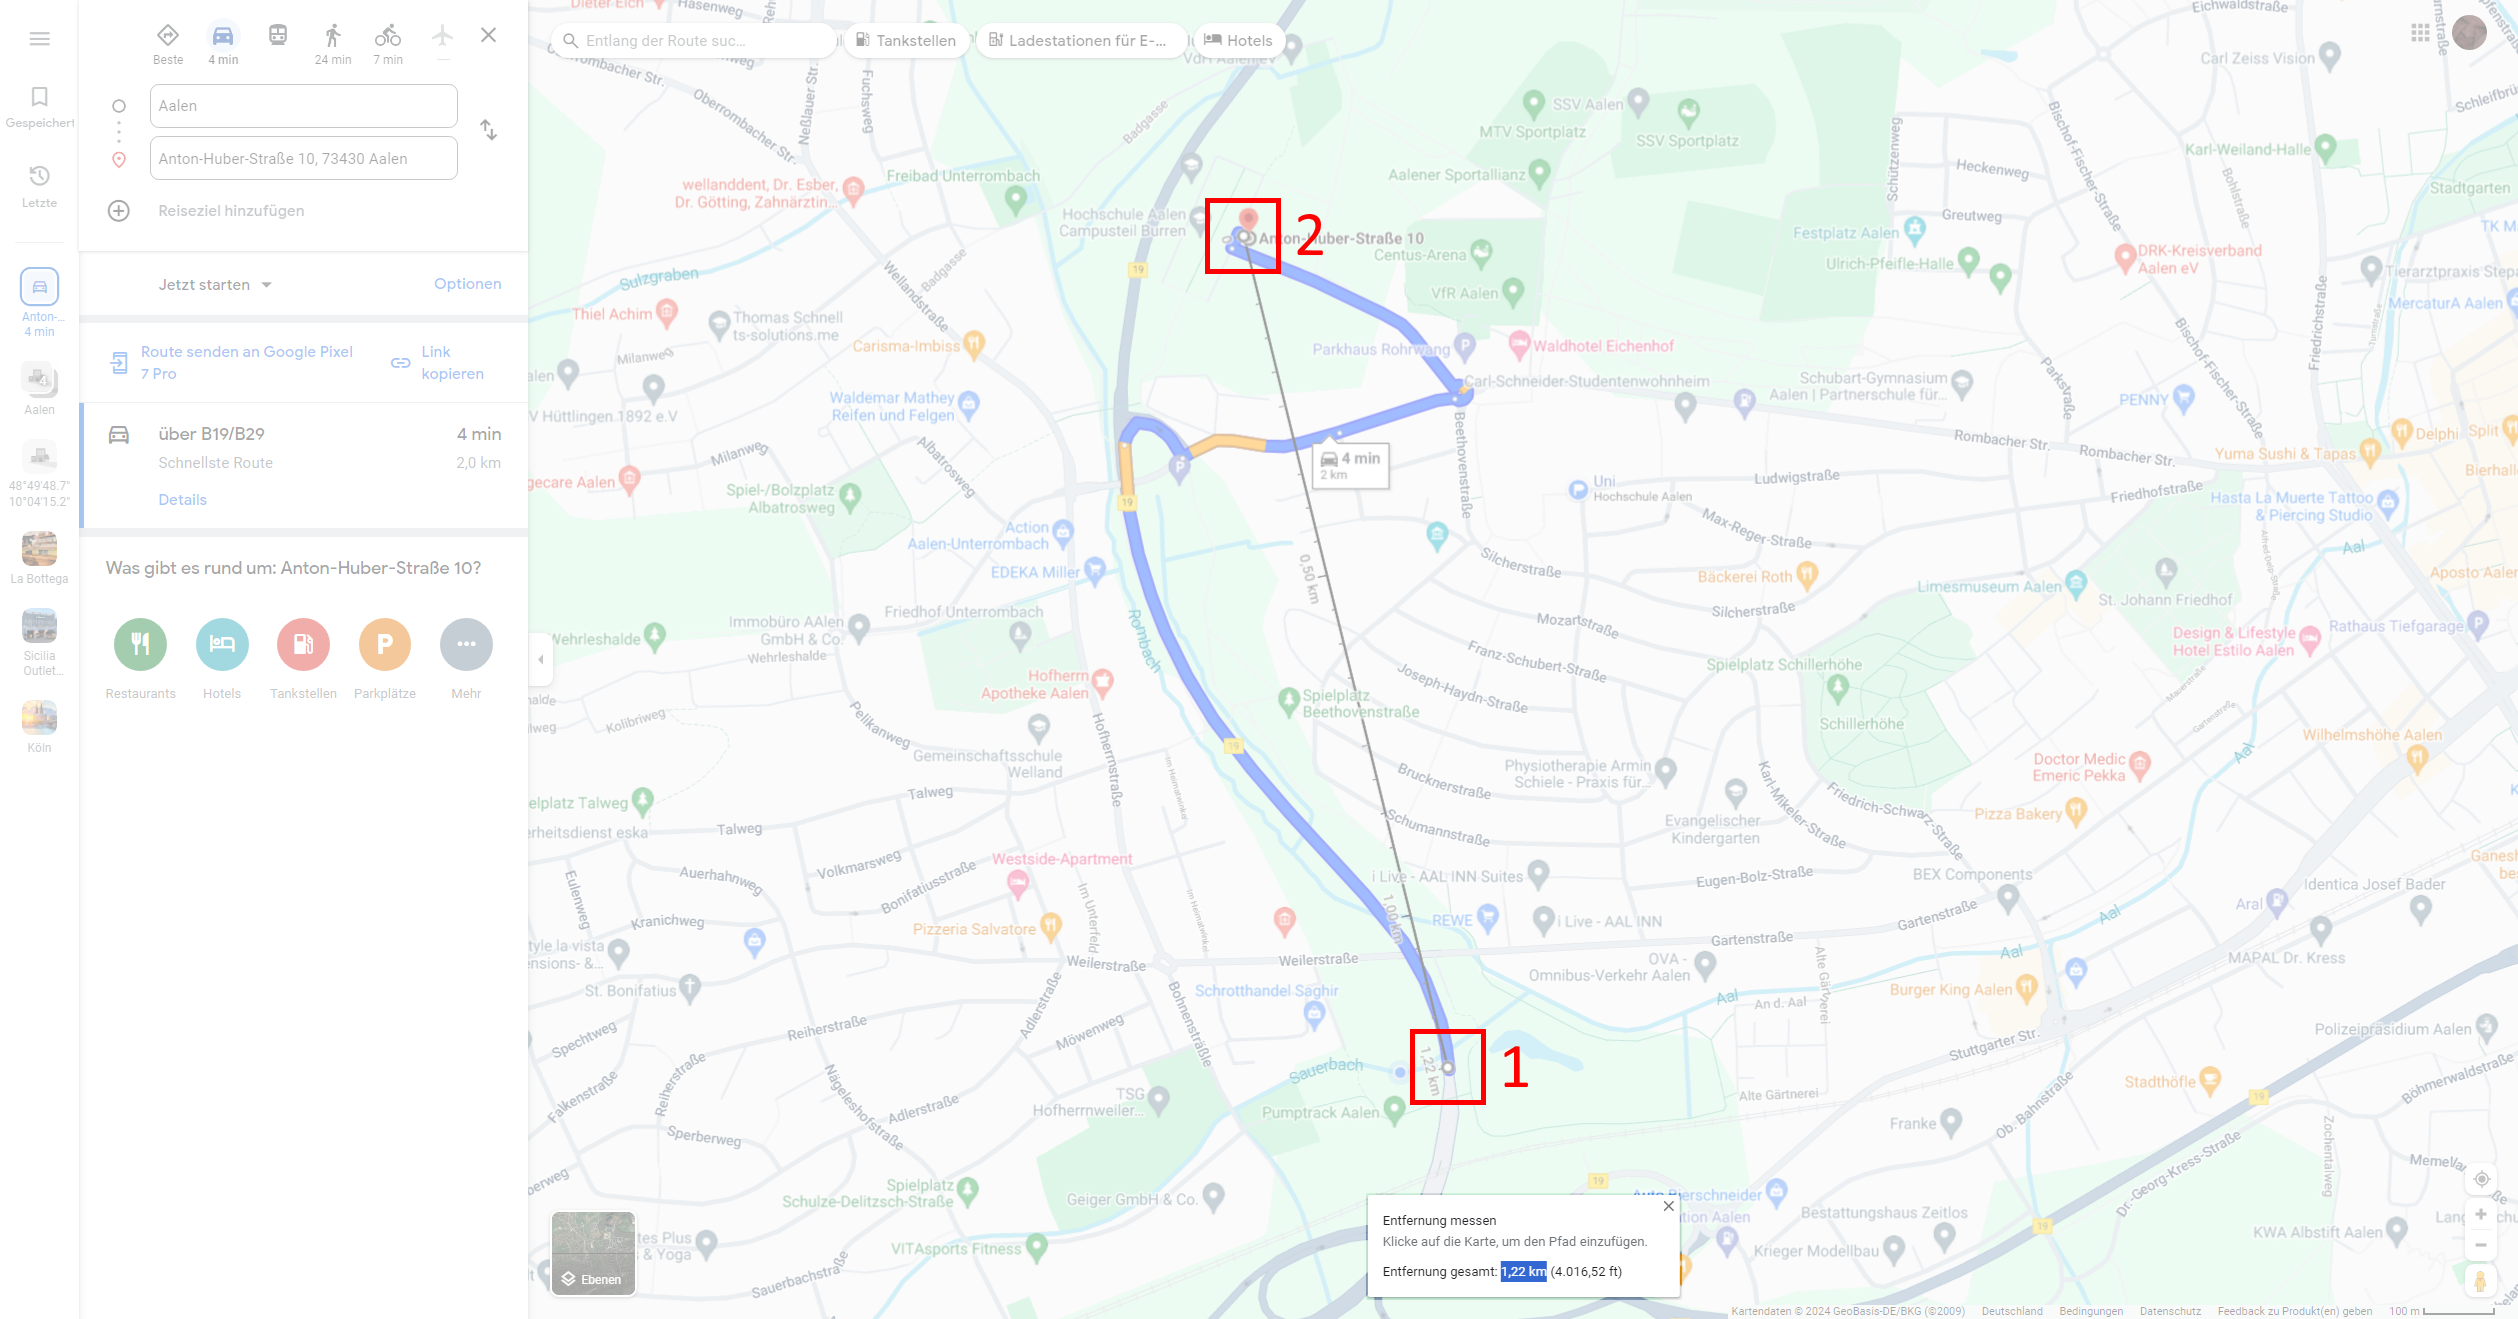
\includegraphics[width=\textwidth]{images/PrAr_Impl_Geolocation-Map.png}
    \caption{Bildschirmabschnitt Abstand Teilnehmer und Lösung}
    \label{fig:implementierung:geolocation_map}
\end{figure}

Abbildung \ref{fig:implementierung:geolocation_map} stellt den Standort des Teilnehmers (Abbildung \ref{fig:implementierung:geolocation_map} - 1) zu einem gesuchten Standort (Abbildung \ref{fig:implementierung:geolocation_map} - 2) dar. Die tatsächliche Distanz entspricht in diesem Beispiel \textit{1213.14} Meter.

\begin{figure}[H]
    \centering
    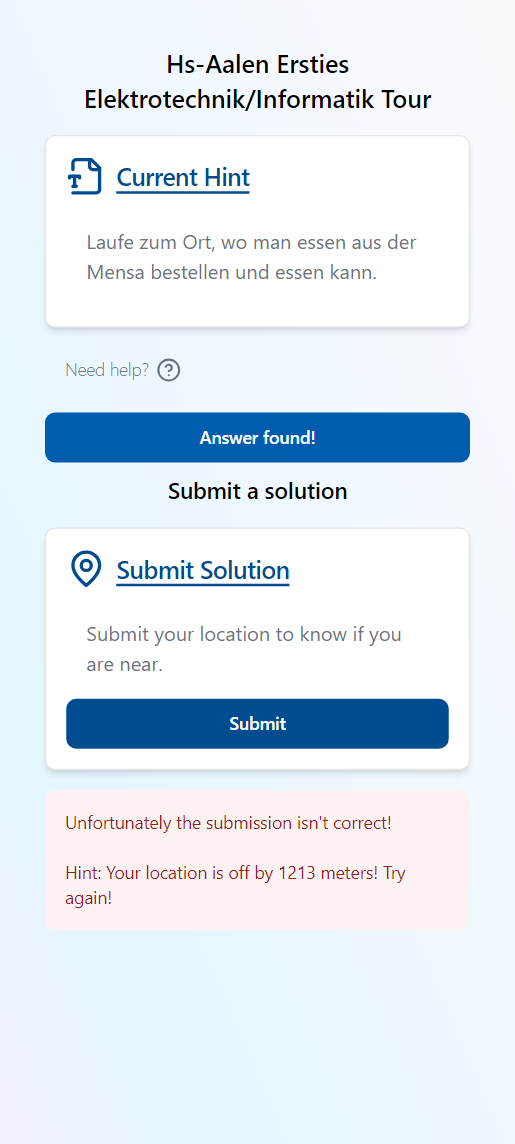
\includegraphics[width=0.5\textwidth]{images/PrAr_Impl_Geolocation-UI.png}
    \caption{Bildschirmabschnitt Abstands-Hinweis an Teilnehmer}
    \label{fig:implementierung:geolocation_ui}
\end{figure}

Abbildung \ref{fig:implementierung:geolocation_ui} zeigt den Zustand der Benutzeroberfläche an, nachdem ein Teilnehmer seine Position als Lösung an das System schickt. Es wurde korrekterweise erkannt, dass der Teilnehmer \textit{1213.14} Meter von der gewollten Lösung entfernt ist.

\subsection{Levenshtein-Algorithmus zur Bestimmung textueller Unterschiede}

Um den Nutzern Feedback darüber zu geben, wie nah ihre eingesandte Antwort an der korrekten Lösung liegt, wird neben der Haversine-Formel auch ein Algorithmus zur Berechnung der Levenshtein-Distanz eingesetzt. Diese Methode wird verwendet, wenn die Lösung aus Textdaten besteht, wie etwa bei der Eingabe von Textantworten auf Rätsel oder Aufgabenstellungen.

Die Levenshtein-Distanz misst den Unterschied zwischen zwei Zeichenketten in Bezug auf die minimale Anzahl von Einfüge-, Lösch- und Ersetzungsoperationen, die erforderlich sind, um die eine Zeichenkette in die andere zu transformieren. Dies ist besonders nützlich, um Tippfehler oder leichte Abweichungen in den Antworten der Nutzer zu identifizieren und entsprechende Rückmeldungen zu geben, die darauf hinweisen, dass die Antwort fast richtig ist, wenn nur geringe Abweichungen vorliegen.

Der folgende C\#-Code zeigt die Implementierung der Levenshtein-Distanz:
\newpage
\begin{lstlisting}[language=c,caption={Code Ausschnitt zum Levenshtein Distanz Algorithmus in C\#}]
public static int LevenshteinDistance(string givenText, string expectedText)
    {
        int n = givenText.Length;
        int m = expectedText.Length;
        int[,] d = new int[n + 1, m + 1];

        // Initialize the distance matrix
        for (int i = 0; i <= n; i++)
        {
            d[i, 0] = i;
        }
        for (int j = 0; j <= m; j++)
        {
            d[0, j] = j;
        }

        // Compute the distances
        for (int i = 1; i <= n; i++)
        {
            for (int j = 1; j <= m; j++)
            {
                int cost = (givenText[i - 1] == expectedText[j - 1]) ? 0 : 1;

                d[i, j] = Math.Min(
                    Math.Min(d[i - 1, j] + 1, d[i, j - 1] + 1),
                    d[i - 1, j - 1] + cost);
            }
        }

        return d[n, m];
    }
\end{lstlisting}
Die Matrix \lstinline{d} wird so initialisiert, dass die ersten Zeilen und Spalten mit aufsteigenden Werten gefüllt sind. Diese Werte entsprechen den Kosten für das Einfügen oder Löschen von Zeichen, um die Länge der anderen Zeichenfolge zu erreichen. Die Hauptlogik des Algorithmus durchläuft die Matrix und berechnet die minimalen Kosten für die Transformation der Teilstrings. Dies geschieht durch Vergleich der aktuellen Zeichen der beiden Zeichenketten und Anwendung der entsprechenden Operationen (Einfügen, Löschen, Ersetzen). Der letzte Wert der Matrix \lstinline{d[n, m]} gibt die minimale Anzahl von Transformationen an, die erforderlich sind, um die beiden Zeichenketten einander anzugleichen.

Die Levenshtein-Distanz ermöglicht es dem System, eine präzise Rückmeldung darüber zu geben, wie nahe der Benutzer an der richtigen Antwort ist, und unterstützt so eine positive Benutzererfahrung durch konstruktives Feedback.

\subsubsection{Anwendungsbeispiel des Levenshtein-Algorithmus}

Im Folgenden wird der Levenshtein-Algorithmus zum Bestimmen der Anzahl an abweichenden Ziffern zu einem gesuchten Lösungstext verwendet.

\begin{figure}[H]
    \centering
    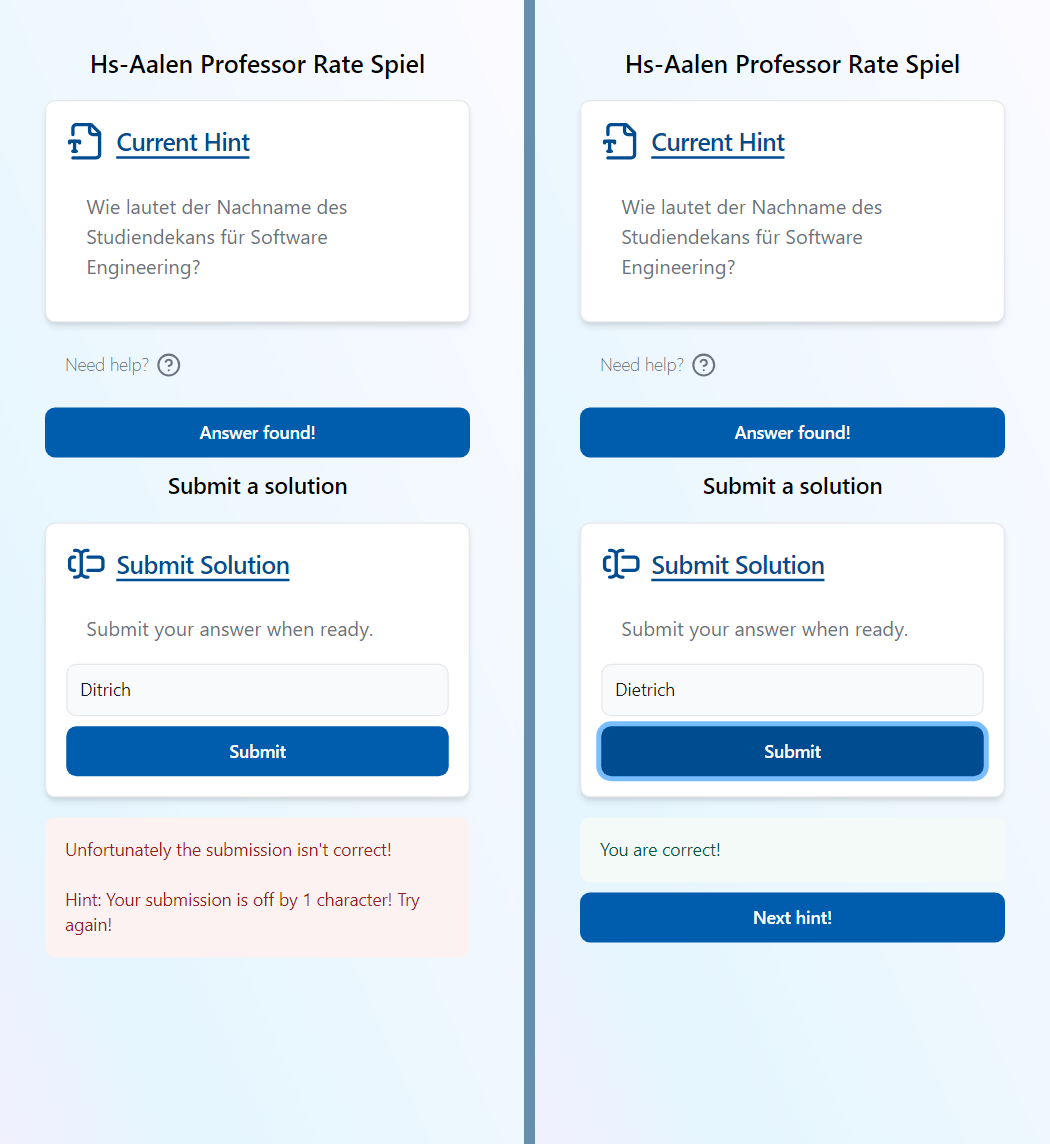
\includegraphics[width=0.75\textwidth]{images/PrAr_Impl_CharacterDiff-UI.png}
    \caption{Bildschirmabschnitte Text Unterschied an Teilnehmer}
    \label{fig:implementierung:characterdiff_ui}
\end{figure}

Der linke Bildschirmabschnitt in Abbildung \ref{fig:implementierung:characterdiff_ui} zeigt den Hinweis, wenn sich ein Teilnehmer in seiner Lösung um eine Ziffer vertan hat. Der rechte Bildschirmabschnitt in Abbildung \ref{fig:implementierung:characterdiff_ui} wird angezeigt, wenn der Benutzer eine korrekte (Text-)Lösung eingegeben hat.


\chapter{Inbetriebnahme} \label{cha:inbetriebnahme}

\section{Einführung}

In diesem Kapitel werden die Maßnahmen für das Deployment der Anwendung näher beschrieben. Anhand einer Übersicht wird gezeigt, wie das System im laufenden Zustand aussieht und wie die unterschiedlichen Anwendungen mit dem Backend interagieren.

\section{Backend Containerisierung}

\begin{figure}[H]
  \centering
  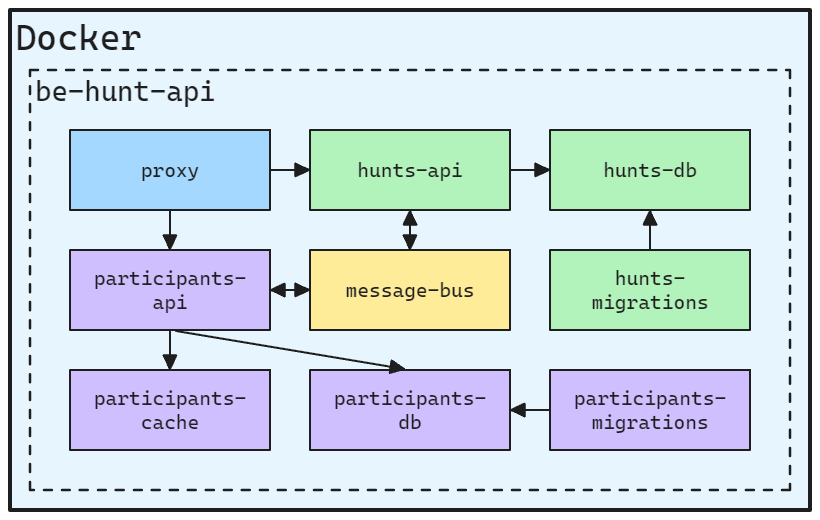
\includegraphics[width=\textwidth]{images/PrAr_Depl_Docker.png}
  \caption{UML-Diagramm für das Deployment}
  \label{fig:deployment:docker}
\end{figure}

Abbildung \ref{fig:deployment:docker} stellt die Deployment-Ansicht des Backends dar. Das Deployment wird durch die Docker Containerisierung ermöglicht (vgl. Kapitel \ref{cha:grundlagen:swtech:docker}). Die Konfiguration der verschiedenen Dienste erfolgt über \textit{Docker-Compose} definiert.

Der Proxy (vgl. Abbildung \ref{fig:deployment:docker} - blau) fungiert als zentraler Einstiegspunkt für die Anwendungen von außen. Er leitet alle Anfragen an den jeweils zuständigen Dienst weiter. Im Falle von falschen oder ungültigen Anfragen wird die Verbindungsanfrage beendet. Die Implementierung und Konfiguration des Proxies ist im Anhang \ref{appendix:code:dockercompose} beschrieben.

Die beiden Container \textit{Participants-Api} und \textit{Hunts-Api} (vgl. Abbildung \ref{fig:deployment:docker} - grün und violett) repräsentieren die deployten Release-Builds der entworfenen Services aus Kapitel \ref{cha:swentwurf:backend}. Diese verfügen jeweils über einen eigenen Datenbank-Container zur persistenten Datenhaltung.

Für die initiale Erstellung und Aktualisierung bestehender Datenbank-Container sind zusätzlich die beiden Migration-Container \textit{Participants-Migrations} und \textit{Hunts-Migrations} vorgesehen (vgl. Abbildung \ref{fig:deployment:docker} - grün und violett). Beide öffnen eine Verbindung zur jeweiligen Datenbank und erstellen die initial benötigten Datenbanktabellen, damit diese für die Verwendung im jeweiligen Service mit den aktuellen Datenbanktabellen existieren.

Die jeweiligen Dockerfiles sind im Anhang näher beschrieben (vgl. Anhang \ref{appendix:code:dockercompose}).

\section{Frontend Containerisierung}

Da das Frontend mit Web-Technologien (vgl. Kapitel \ref{cha:grundlagen:swtech:svelte}) implementiert wurde, kann es als plattformunabhängige Browseranwendung auf einem Webserver deployt werden. Dies ist auch über Docker Containerisierung möglich, wurde aber im Rahmen des Projektes nicht entworfen und getestet.

Für das Deployment der Hunt-Editor Web-App für Desktops wäre es auch möglich, eine echte Anwendung daraus zu machen. Hierfür stehen bereits implementierte Technologien wie \textit{Tauri} zur Verfügung (siehe \autocite{github:tauri} und \autocite{tauri:tauri}).


\chapter{Zusammenfassung und Ausblick}
\label{cha:zusammenfassung}

\section{Erreichte Ergebnisse}
\label{sec:ergebnisse}

Die Zusammenfassung dient dazu, die wesentlichen Ergebnisse des 
Praktikums und vor allem die entwickelte Problemlösung und den 
erreichten Fortschritt darzustellen. (Sie haben Ihr Ziel erreicht und 
dies nachgewiesen).

\section{Ausblick}
\label{sec:ausblick}

Im Ausblick werden Ideen für die Weiterentwicklung der erstellten Lösung 
aufgezeigt. Der Ausblick sollte daher zeigen, dass die Ergebnisse der 
Arbeit nicht nur für die in der Arbeit identifizierten Problemstellungen 
verwendbar sind, sondern darüber hinaus erweitert sowie auf andere 
Probleme übertragen werden können.

\subsection{Erweiterbarkeit der Ergebnisse}
\label{sub:erweiterbarkeit}

Hier kann man was über die Erweiterbarkeit der Ergebnisse sagen.

\subsection{Übertragbarkeit der Ergebnisse}
\label{sub:uebertragbarkeit}

Und hier etwas über deren Übertragbarkeit.

%-----------------------------------------------------------------------
%----- LITERATUR & ANHANG ----------------------------------------------
\appendix
\printbibliography[heading=bibintoc]

\chapter{Anhang: Entscheidungen bei der Implementierung}

\section{Architektonische Entscheidungen}

\subsection{Wahl eines Message-Bus für das Hunt-Api Backend}

% TODO: Beschreiben was für ein grund das hat, aka nicht valide teilnahmen erkennen.

\subsection{Wahl eines Api-Gateways für das Hunt-Api Backend}

% TODO: Beschreiben was das auf sich hat, aka nicht services einzelnd pingen aber einheitliche schnittstelle + eventuelle service sicherheit die später kommt durch sonder headers and stuff wenn wir das machen aber architektonisch einfach bessere wahl, ja der text macht grad wenig sinn weil ich aus irgwend nem grund irgendwas tippen will, bitte lächeln 

\subsection{Hinweise und Lösungen ohne Abstrakte Klassen} \label{appendix:adr:er}

\subsubsection{Kontext}

Für das Speichern der Aufgaben (\textit{Assignments}) einer Schnitzeljagd soll es möglich sein, aus unterschiedlichen Arten von Hinweisen (\textit{Hints}) und Lösungen (\textit{Solutions}) zu wählen.

\subsubsection{Entscheidung}

Statt für jeden Hinweis-Typ und Lösungs-Typ unterschiedliche abstrakte Datenklassen zu definieren, werden diese lediglich als Daten-String gespeichert.

\subsubsection{Begründung}

Es wurde im Rahmen der Projektdurchführung versucht, mit abstrakten Datenklassen zu arbeiten. Jedoch erhöht dies die Komplexität enorm.

Zudem ist diese Lösung nicht skalierbar, denn es wird mehr Aufwand erfordert, einen neuen Hinweis-Typ oder Lösungs-Typ in das System einzubauen. Zunächst muss eine neue Datenklasse definiert werden, Dann muss diese in das Datenbank-Modell als konkrete neue Tabelle eingefügt werden.

In den meisten Fällen unterscheiden sich die Hinweis-Typen oder Lösungs-Typen kaum am Datenformat. Texte oder Bilder werden im System als String gespeichert. Daher entspringt die zentrale Frage: Wieso überhaupt mit abstrakten Klassen alles verkomplizieren?

\subsubsection{Konsequenzen}

\begin{itemize}
    \item \textbf{Keine Type-Safety}: Geo-Locations im Format \textit{lat;lon} werden als verketteter String gespeichert und müssen beim Ausleseprozess jeweils umgewandelt werden, was sehr fehleranfällig ist.
\end{itemize}

\section{Entscheidungen im Frontend}

\subsection{Wahl von Flowbite statt DaisyUI} \label{appendix:adr:daisy}

\subsubsection{Unterschied zwischen Flowbite-Svelte und DaisyUI}

\textbf{DaisyUI} ist eine Komponentenbibliothek für Tailwind CSS, die eine Vielzahl von vorgefertigten UI-Komponenten bereitstellt. Es ist darauf ausgelegt, die Nutzung von Tailwind CSS zu vereinfachen, indem es gebrauchsfertige Klassen und Designs bietet. DaisyUI ist besonders bekannt für seine einfache Integration und die Möglichkeit, schnell und effizient ästhetisch ansprechende Benutzeroberflächen zu erstellen, ohne viel eigene CSS-Regeln schreiben zu müssen. 

Im Folgenden ein Beispiel für die Verwendung von DaisyUI, um ein Modal zu erstellen:

\begin{lstlisting}[language=html, caption={Code Ausschnitt DaisyUI Beispiel}]
<button class="btn" onclick="my_modal_1.showModal()">open modal</button>
<dialog id="my_modal_1" class="modal">
  <div class="modal-box">
    <h3 class="text-lg font-bold">Hello!</h3>
    <p class="py-4">Press ESC key or click the button below to close</p>
    <div class="modal-action">
      <form method="dialog">
        <!-- if there is a button in form, it will close the modal -->
        <button class="btn">Close</button>
      </form>
    </div>
  </div>
</dialog>
\end{lstlisting}

\textbf{Flowbite-Svelte} ist eine auf Tailwind CSS basierende UI-Komponentenbibliothek, die speziell für die Integration mit Svelte entwickelt wurde. Sie bietet eine umfassende Sammlung von UI-Komponenten wie Buttons, Modale, Formulare und vieles mehr. Flowbite-Svelte kombiniert die Leistungsfähigkeit von Tailwind CSS mit der reaktiven Natur von Svelte, um die Entwicklung dynamischer und interaktiver Webanwendungen zu erleichtern. Zudem bietet Flowbite-Svelte eine nahtlose Svelte-Integration, was bedeutet, dass die Komponenten als echte Svelte-Komponenten bereitgestellt werden, die sich perfekt in das Svelte-Ökosystem einfügen. 

Im Folgenden ein Beispiel für die Verwendung von Flowbite-Svelte, das das gleiche Modal erstellt wie im DaisyUI-Beispiel:

\begin{lstlisting}[language=html, caption={Code Ausschnitt Flowbite-Svelte Beispiel}]
<script>
  import { Button, Modal } from 'flowbite-svelte';
  let defaultModal = false;
</script>

<Button on:click={() => (defaultModal = true)}>open modal</Button>
<Modal title="Hello!" bind:open={defaultModal} autoclose>
  <p class="text-base leading-relaxed text-gray-500 dark:text-gray-400">Press ESC key or click the button below to close</p>
  <svelte:fragment slot="footer">
    <Button on:click={() => (defaultModal = false)}>Close</Button>
  </svelte:fragment>
</Modal>
\end{lstlisting}

\subsubsection{Begründung für den Wechsel zu Flowbite-Svelte}

Der Wechsel von DaisyUI zu Flowbite-Svelte ist aus mehreren Gründen gerechtfertigt. Erstens bietet Flowbite-Svelte eine speziell auf Svelte abgestimmte Komponentenbibliothek, die eine engere und effizientere Integration ermöglicht. Dies bedeutet, dass die UI-Komponenten in Flowbite-Svelte als native Svelte-Komponenten verfügbar sind, was die Entwicklungsarbeit vereinfacht und die Nutzung von Svelte-spezifischen Features erleichtert.

Zweitens ist die Anpassungsfähigkeit und Erweiterbarkeit von Flowbite-Svelte ein wesentlicher Vorteil. Während DaisyUI zwar eine einfache Möglichkeit bietet, Tailwind CSS zu nutzen, ist Flowbite-Svelte besser darauf ausgelegt, komplexere und dynamischere Benutzeroberflächen zu unterstützen. Dies ist besonders wichtig für eine Anwendung wie den Schnitzeljagd-Editor, die eine hohe Interaktivität und eine benutzerfreundliche Oberfläche erfordert.

Darüber hinaus bietet Flowbite-Svelte eine breitere Palette an vorgefertigten Komponenten und Layout-Optionen, was die Entwicklung beschleunigt und gleichzeitig die Konsistenz und Qualität der Benutzeroberfläche verbessert. Dies trägt dazu bei, dass die Anwendung nicht nur funktional, sondern auch optisch ansprechend und intuitiv zu bedienen ist.

\chapter{Anhang: Code Abschnitte}

\section{Inbetriebnahme}

\subsection{Docker-Compose für das Backend} \label{appendix:code:dockercompose}

% TODO

\end{document}